\documentclass[a4paper, 12pt]{article}

\usepackage{polski}
\usepackage[utf8]{inputenc}
\usepackage{a4wide}
\usepackage[OT4]{fontenc}
\usepackage[english,polish]{babel}
\usepackage{indentfirst}
\usepackage{graphicx} 
\usepackage{float}
\usepackage{hhline}
\usepackage{multirow}
\usepackage{geometry}
\usepackage{color}
\usepackage{multirow}
\usepackage{enumerate}
\usepackage{pdfpages}
\usepackage[table,xcdraw]{xcolor}
\usepackage[normalem]{ulem}
\usepackage[hidelinks, pdftoolbar = false, pdfmenubar = false, bookmarks = false]{hyperref}

\useunder{\uline}{\ul}{}

\renewcommand{\baselinestretch}{1.5}

\newgeometry{tmargin=2.cm, bmargin=2cm, lmargin=0.5cm, rmargin=0.5cm} 

\begin{document}

\thispagestyle{empty}
\noindent Grzegorz Suszka, indeks: 218292 \hfill Wrocław, dn.\ \today \\ Daniel Rupek, indeks: 218143 \\

\vfill

\begin{center}
  \begin{Huge}
  	Technologie sieciowe 2 - projekt \\
  \end{Huge}  
\end{center}

\begin{center}
  Rok akad. 2016/2017, kierunek: INF
\end{center}

\vspace{0.2ex}

\begin{flushright}
	\begin{minipage}[t]{0.4\columnwidth}
	\noindent Prowadzący:\\ dr inż. Marcin Markowski
	\end{minipage}
\end{flushright}

\vfill
\newpage
\tableofcontents
\listoftables
\vfill
\newpage

\section{Etap 1}

\subsection{Wstęp}

Celem projektu jest zaprojektowanie sieci komputerowej dla biura projektowego \emph{Agusto}. Firma zajmuje się tworzeniem kompleksowych projektów budynków (zarówno użytkowych, jak i mieszkalnych) dostosowanych do indywidualnych potrzeb klientów. W związku z szybkim rozwojem firmy nastąpiła potrzeba zmiany siedziby z powodu zbyt dużej liczby pracowników. Wcześniejsza siedziba firmy znajdowała się w obszarze mieszkalnym, tak więc znalezienie pobliskiego budynku z wolną przestrzenią było niemożliwe. Zdecydowano, że nowa siedziba firmy mieścić będzie się w Wrocławiu, w dwóch budynkach oddalonych od siebie o 100 metrów.\\

Projekt sieci komputerowej powinien uwzględnić następujące potrzeby biura projektowego \emph{Agusto}

\begin{enumerate}[a)]

	\item możliwość zarządzania większymi projektami dzięki systemowi kontroli wersji
	
	\item możliwość prowadzenia wideokonferencji ze zleceniodawcami w celu konsultacji postępów dokonanych w realizacji projektu, bądź też konferencji wewnątrzprojektowych poprzez komunikator Skype for Business, w celu sprawniejszej realizacji zadań składających się na projekt
	
	\item możliwość komunikacji z podwykonawcami poprzez e-mail, VoIP, bądź komunikator Skype for Business
	
\end{enumerate}

\subsection{Inwentaryzacja zasobów, sprzętu, aplikacji, zasobów ludzkich}

\begin{table}[H]
	\centering
	\begin{tabular}{l|c|c|c|c|c|}
	\cline{2-6}
	\multirow{2}{*}{}                   & \multicolumn{5}{c|}{\textbf{Liczba użytkowników (komputerów)}} \\ \cline{2-6} 
	                                    & \multicolumn{3}{c|}{\textbf{Budynek 1}}  & \multicolumn{2}{c|}{\textbf{Budynek 2}} \\ \hline
	\multicolumn{1}{|c|}{\textbf{Grupa robocza}} & \textbf{Piętro 1}  & \textbf{Piętro 2} & \textbf{Piętro 3} & \textbf{Piętro 1}       & \textbf{Piętro 2}      \\ \hline
	\multicolumn{1}{|c|}{\textbf{Konstruktorzy}} & 12        & 5        & 4        & 9              & 7             \\ \hline
	\multicolumn{1}{|c|}{\textbf{Architekci}}    & 14        & 20       & 32       & 32             & 18            \\ \hline
	\multicolumn{1}{|c|}{\textbf{Projektanci}}   & 5         & 1        & 35       & 21             & 15            \\ \hline
	\multicolumn{1}{|c|}{\textbf{Zarząd}}        & 14        & 2        & 28       & 1              & 5             \\ \hline
	\multicolumn{1}{|c|}{\textbf{Praktykanci}}   & 17        & 11       & 29       & 15             & 16            \\ \hline
	\multirow{6}{*}{}                   & \multicolumn{5}{l|}{\textbf{Liczba drukarek}}                             \\ \cline{2-6} 
	                                    & 2         & 3        & 2        & 2              & 1             \\ \cline{2-6} 
	                                    & \multicolumn{5}{l|}{\textbf{Liczba punktów dostępowych Wi-Fi}}            \\ \cline{2-6} 
	                                    & 0         & 1        & 0        & 0              & 3             \\ \cline{2-6} 
	                                    & \multicolumn{5}{l|}{\textbf{Liczba urządzeń bezprzewodowych}}             \\ \cline{2-6} 
	                                    & 0         & 16       & 0        & 0              & 9             \\ \cline{2-6} 
	\end{tabular}
	\caption{Rozstawienie urządzeń w budynkach}
\end{table}

\begin{table}[H]
	\centering
	\begin{tabular}{|c|c|c|}
	\hline
	\multicolumn{3}{|c|}{\textbf{Punkty dystrybucyjne}}                 \\ \hline
	\textbf{Oznaczenie}            & \multicolumn{2}{l|}{\textbf{Lokalizacja}}   \\ \hline
	\multirow{2}{*}{\textbf{MDF}}  & Bud. 1   & Bud. 1                  \\
	                      & Piętro 1 & Piętro 1                \\ \hline
	\multirow{2}{*}{\textbf{IDF1}} & Bud. 1   & Bud. 1                  \\
	                      & Piętro 2 & Piętro 2, 3             \\ \hline
	\multirow{2}{*}{\textbf{IDF2}} & Bud. 2   & \multirow{2}{*}{Bud. 2} \\
	                      & Piętro 2 &                         \\ \hline
	\end{tabular}
	\caption{Rozstawienie punktów dystrybucyjnych}
\end{table}

\begin{table}[H]
	\centering
	\begin{tabular}{l|c|c|c|}
	\cline{2-4}
	                                    & \multicolumn{3}{c|}{\textbf{Serwer (download/upload) {[}kbps{]}}} \\ \hline
	\multicolumn{1}{|c|}{\textbf{Grupa rob.}}    & \textbf{Serwer 1}       & \textbf{Serwer 2}        & \textbf{Drukarka}       \\ \hline
	\multicolumn{1}{|c|}{\textbf{Konstruktorzy}} & 350/650           & 590/950           & 10/120           \\ \hline
	\multicolumn{1}{|c|}{\textbf{Architekci} }   & 300/150           & 100/850           & 10/200           \\ \hline
	\multicolumn{1}{|c|}{\textbf{Projektanci}}   & 500/950           & 650/100           & 10/180           \\ \hline
	\multicolumn{1}{|c|}{\textbf{Zarząd} }       & 450/500           & 700/700           & 10/180           \\ \hline
	\multicolumn{1}{|c|}{\textbf{Praktykanci}}   & 150/650           & 400/850           & 10/190           \\ \hline
	\multicolumn{1}{|c|}{\textbf{Wi-Fi}}         & 100/200           & 0/0               & 10/150           \\ \hline
	\end{tabular}
	\caption{Transfer serwerów lokalnych i drukarek}
\end{table}

\begin{table}[H]
	\centering
	\begin{tabular}{l|c|c|c|}
	\cline{2-4}
	                                          & \multicolumn{3}{l|}{\begin{tabular}[c]{@{}l@{}}\textbf{Transfer do/z Internetu na jedną sesję (internautę) [kbps]}\end{tabular}} \\ \hline
	\multicolumn{1}{|c|}{\textbf{Serwery internetowe}} & \textbf{Do Internetu}         & \textbf{Z Internetu}         & \begin{tabular}[c]{@{}l@{}}\textbf{Liczba jednoczesnych sesji}\end{tabular}         \\ \hline
	\multicolumn{1}{|c|}{\textbf{Serwer WWW}}          & 120                  & 15                  & 34                                                                           \\ \hline
	\multicolumn{1}{|c|}{\textbf{Serwer FTP}}          & 220                  & 60                  & 17                                                                           \\ \hline
	\end{tabular}
	\caption{Transfer serwerów WWW i FTP}
\end{table}

\begin{table}[H]
	\centering
	\resizebox{17cm}{!}{
	\begin{tabular}{l|c|c|c|c|c|c|}
	\cline{2-7}
	                                    & \multicolumn{6}{c|}{\textbf{Transfer z/do Internetu (download/upload) {[}kbps{]}}}            \\ \hline
	\multicolumn{1}{|c|}{\textbf{Grupa rob.}}    & \textbf{Przeglądarka} & \textbf{Wideokonferencja} & \textbf{VoIP}  & \textbf{Klient FTP} & \textbf{Komunikator} & \textbf{Praca w chmurze} \\ \hline
	\multicolumn{1}{|c|}{\textbf{Konstruktorzy}} & 58/10        & 40/40            & 20/20 & 55/11      & 0/0         & 0/0             \\ \hline
	\multicolumn{1}{|c|}{\textbf{Architekci}}    & 0/0          & 40/40            & 20/20 & 0/0        & 0/0         & 0/0             \\ \hline
	\multicolumn{1}{|c|}{\textbf{Projektanci}}   & 61/10        & 40/40            & 20/20 & 95/12      & 0/0         & 31/50           \\ \hline
	\multicolumn{1}{|c|}{\textbf{Zarząd}}        & 0/0          & 40/40            & 0/0   & 0/0        & 15/15       & 57/43           \\ \hline
	\multicolumn{1}{|c|}{\textbf{Praktykanci}}   & 49/10        & 0/0              & 0/0   & 0/0        & 15/15       & 25/21           \\ \hline
	\multicolumn{1}{|c|}{\textbf{Wi-Fi}}         & 0/0          & 40/40            & 20/20 & 89/12      & 15/15       & 0/0             \\ \hline
	\end{tabular}}
	\caption{Transfer Internetu w aplikacjach}
\end{table}

Na podstawie podanych przez Prowadzącego danych można wywnioskować, że potrzeby poszczególnych grup roboczych są zróżnicowane. Z przeglądarki korzystają w podobnym stopniu wszyscy oprócz architektów oraz zarządu, co generuje relatywnie wysoki transfer danych. Podobnie, z wideokonferencji korzystają prawie wszystkie grupy, wyjątkiem są praktykanci, którym nie biorą udziału w kontakcie ze zleceniodawcą. Korzystanie z technologii VoIP generuje stosunkowo niski transfer danych. Klient FTP powoduje wysoki download danych, jednak korzystają z niego głównie konstruktorzy oraz projektanci. Z komunikatora korzystają grupy robocze, które nie korzystają z technologii VoIP. Do pracy w chmurze wykorzystywany jest średni transfer, przy czym w większości generowany jest on przez zarząd, który sprawuje kontrolę nad poprawnością wykonania projektu. Grupa WiFi, która oznacza w tym przypadku prywatne, bądź służbowe urządzenia pracowników, którzy łączą się z siecią w sposób bezprzewodowy, generuje transfer głównie przy pobieraniu danych z FTP.

\subsection{Analiza potrzeb użytkowników - wymagania zamawiającego}
\begin{itemize}
	\item Ruch w sieci lokalnej:
	
\begin{table}[H]
\centering
\resizebox{17cm}{!}{
\begin{tabular}{c|c|c|c|c|}
\hline
\multicolumn{5}{|c|}{\textbf{Budynek 1}}                                                                                                                             \\ \hline
\textbf{}                                    & \multicolumn{2}{c|}{\textbf{Serwer 1}}                    & \multicolumn{2}{c|}{\textbf{Serwer 2}}                    \\ \hline
\multicolumn{1}{|c|}{\textbf{Grupa robocza}} & \textbf{download {[}kbps{]}} & \textbf{upload {[}kbps{]}} & \textbf{download {[}kbps{]}} & \textbf{upload {[}kbps{]}} \\ \hline
\multicolumn{5}{|c|}{\textbf{Piętro 1}}                                                                                                                              \\ \hline
\multicolumn{1}{|c|}{\textbf{Konstruktorzy}} & 4200                         & 7800                       & 7800                         & 11400                      \\ \hline
\multicolumn{1}{|c|}{\textbf{Architekci}}    & 4200                         & 2100                       & 1400                         & 11900                      \\ \hline
\multicolumn{1}{|c|}{\textbf{Projektanci}}   & 2500                         & 4750                       & 3250                         & 500                        \\ \hline
\multicolumn{1}{|c|}{\textbf{Zarząd}}        & 6300                         & 7000                       & 9800                         & 9800                       \\ \hline
\multicolumn{1}{|c|}{\textbf{Praktykanci}}   & 2550                         & 11050                      & 6800                         & 14450                      \\ \hline
\multicolumn{1}{|c|}{{\ul \textbf{Suma}}}    & 19750                        & 32700                      & 29050                        & 48050                      \\ \hline
\multicolumn{5}{|c|}{\textbf{Piętro 2}}                                                                                                                              \\ \hline
\multicolumn{1}{|c|}{\textbf{Konstruktorzy}} & 1750                         & 3250                       & 3250                         & 4750                       \\ \hline
\multicolumn{1}{|c|}{\textbf{Architekci}}    & 6000                         & 3000                       & 2000                         & 17000                      \\ \hline
\multicolumn{1}{|c|}{\textbf{Projektanci}}   & 500                          & 950                        & 650                          & 100                        \\ \hline
\multicolumn{1}{|c|}{\textbf{Zarząd}}        & 900                          & 1000                       & 1400                         & 1400                       \\ \hline
\multicolumn{1}{|c|}{\textbf{Praktykanci}}   & 1650                         & 7150                       & 4400                         & 9350                       \\ \hline
\multicolumn{1}{|c|}{{\ul \textbf{Suma}}}    & 10800                        & 15350                      & 11700                        & 32600                      \\ \hline
\multicolumn{5}{|c|}{\textbf{Piętro 3}}                                                                                                                              \\ \hline
\multicolumn{1}{|c|}{\textbf{Konstruktorzy}} & 1400                         & 2600                       & 2600                         & 3800                       \\ \hline
\multicolumn{1}{|c|}{\textbf{Architekci}}    & 9600                         & 4800                       & 3200                         & 27200                      \\ \hline
\multicolumn{1}{|c|}{\textbf{Projektanci}}   & 17500                        & 33250                      & 22750                        & 3500                       \\ \hline
\multicolumn{1}{|c|}{\textbf{Zarząd}}        & 12600                        & 14000                      & 19600                        & 19600                      \\ \hline
\multicolumn{1}{|c|}{\textbf{Praktykanci}}   & 4350                         & 18850                      & 11600                        & 24650                      \\ \hline
\multicolumn{1}{|c|}{{\ul \textbf{Suma}}}    & 45450                        & 73500                      & 59750                        & 78750                      \\ \hline
\end{tabular}}
\caption{Transfer serwerów w budynku pierwszym}
\end{table}

\begin{table}[H]
	\centering
	\begin{tabular}{c|c|c|c|c|}
\hline
\multicolumn{5}{|c|}{\textbf{Budynek 2}}                                                                                                                             \\ \hline
\textbf{}                                    & \multicolumn{2}{c|}{\textbf{Serwer 1}}                    & \multicolumn{2}{c|}{\textbf{Serwer 2}}                    \\ \hline
\multicolumn{1}{|c|}{\textbf{Grupa robocza}} & \textbf{download {[}kbps{]}} & \textbf{upload {[}kbps{]}} & \textbf{download {[}kbps{]}} & \textbf{upload {[}kbps{]}} \\ \hline
\multicolumn{5}{|c|}{\textbf{Piętro 1}}                                                                                                                              \\ \hline
\multicolumn{1}{|c|}{\textbf{Konstruktorzy}} & 3150                         & 5850                       & 5850                         & 8550                       \\ \hline
\multicolumn{1}{|c|}{\textbf{Architekci}}    & 9600                         & 4800                       & 3200                         & 27200                      \\ \hline
\multicolumn{1}{|c|}{\textbf{Projektanci}}   & 10500                        & 19950                      & 13650                        & 2100                       \\ \hline
\multicolumn{1}{|c|}{\textbf{Zarząd}}        & 450                          & 500                        & 700                          & 700                        \\ \hline
\multicolumn{1}{|c|}{\textbf{Praktykanci}}   & 2250                         & 9750                       & 6000                         & 12750                      \\ \hline
\multicolumn{1}{|c|}{{\ul \textbf{Suma}}}    & 25950                        & 40850                      & 29400                        & 51300                      \\ \hline
\multicolumn{5}{|c|}{\textbf{Piętro 2}}                                                                                                                              \\ \hline
\multicolumn{1}{|c|}{\textbf{Konstruktorzy}} & 2450                         & 4550                       & 4550                         & 6650                       \\ \hline
\multicolumn{1}{|c|}{\textbf{Architekci}}    & 5400                         & 2700                       & 1800                         & 15300                      \\ \hline
\multicolumn{1}{|c|}{\textbf{Projektanci}}   & 7500                         & 14250                      & 9750                         & 1500                       \\ \hline
\multicolumn{1}{|c|}{\textbf{Zarząd}}        & 2250                         & 2500                       & 3500                         & 3500                       \\ \hline
\multicolumn{1}{|c|}{\textbf{Praktykanci}}   & 2400                         & 10400                      & 6400                         & 13600                      \\ \hline
\multicolumn{1}{|c|}{{\ul \textbf{Suma}}}    & 20000                        & 34400                      & 26000                        & 40550                      \\ \hline
\end{tabular}
	\caption{Transfer serwerów w budynku drugim}
\end{table}

\noindent \textit{Przykładowe obliczenia dla tablicy 6 i 7:}\\
Dla bud. 1, piętra 1, serwera 1, grupy rob.: konstruktorzy:\\
\(liczba\_konstruktorów\_na\_piętrze\_1\ (tab.\ 1)\ \cdot\ download\_serwera\_1\ (tab.\ 3) = 12\ \cdot\ 350\ kbps = 4200\ kbps\)\\

\begin{table}[H]
	\centering
	\begin{tabular}{c|c|c|}
\cline{2-3}
                                                     & \textbf{Do internetu} & \textbf{Z internetu} \\ \hline
\multicolumn{1}{|c|}{\textbf{Serwer WWW}}                     & 4080         & 510         \\ \hline
\multicolumn{1}{|c|}{\textbf{Serwer FTP}}                     & 3740         & 1020        \\ \hline
\multicolumn{1}{|c|}{{\ul \textbf{Suma {[}kbps{]}}}} & 7820         & 1530        \\ \hline
\multicolumn{1}{|c|}{{\ul \textbf{Suma {[}Mbps{]}}}} & 7,64         & 1,49        \\ \hline
\end{tabular}
	\caption{Łączny transfer serwerów WWW i FTP}
\end{table}

\noindent \textit{Przykładowe obliczenia dla tab. 8:}\\
Dla serwera WWW, do Internetu:\\
\(liczba\_jednoczesnych\_sesji\_WWW\ (tab.\ 4)\ \cdot\ transfer\_WWW\_do\_Internetu\ (tab.\ 4) = 34\ \cdot\ 120\ kbps = 4080\ kbps\)\\


\begin{table}[H]
	\centering
\begin{tabular}{|c|c|c|c|c|}
\hline
                    & \textbf{Download {[}kbps{]}} & \textbf{Upload {[}kbps{]}} & \textbf{Download {[}Mbps{]}} & \textbf{Upload {[}Mbps{]}} \\ \hline
\textbf{Serwer 1}   & 121950                       & 196800                     & 119,09                       & 192,19                     \\ \hline
\textbf{Serwer 2}   & 155900                       & 251250                     & 152,25                       & 245,36                     \\ \hline
\textbf{Drukarki}   & 100                          & 2000                       & 0,10                         & 1,95                       \\ \hline
{\ul \textbf{Suma}} & 277050                       & 452050                     & 271,44                       & 439,50                     \\ \hline
\end{tabular}
	\caption{Łączny transfer sieci lokalnej}
\end{table}
	
\noindent \textit{Przykładowe obliczenia dla tab. 9:}\\
Dla serwera 1, download [Mbps]\\
\(\frac{suma\_transferu\_down\_serwer\_1\ tab.\ (6\ i\ 7)}{1024} =\frac{19750+10800+45450+25950+20000\ kbps}{1024} = 119,09\ Mbps\)\\
	
\item Wykorzystanie sieci Internet:
\begin{table}[H]
\centering
\resizebox{20cm}{!}{
\begin{tabular}{c|c|c|c|c|c|c|c|c|c|c|c|c|l}
\multicolumn{13}{c}{\textbf{Budynek 1}}\\
\cline{1-13}
                                                   & \multicolumn{6}{c|}{\textbf{Download {[}kbps{]}}}                                                                                           & \multicolumn{6}{c|}{\textbf{Upload {[}kbps{]}}}                                                                                           &  \\ \cline{1-13}
\multicolumn{1}{|c|}{\textbf{Grupa robocza}}       & \textbf{Przeglądarka} & \textbf{Wideokonferencja} & \textbf{VoIP} & \textbf{Klient FTP} & \textbf{Komunikator} & \textbf{Praca\_w\_chmurze} & \textbf{Przeglądarka} & \textbf{Wideokonferencja} & \textbf{VoIP} & \textbf{Klient FTP} & \textbf{Komunikator} & \textbf{Praca w chmurze} &  \\ \cline{1-13}
\multicolumn{1}{|c|}{\textbf{Konstruktorzy}}       & 1218                  & 840                       & 420           & 1155                & 0                    & 0                          & 210                   & 840                       & 420           & 231                 & 0                    & 0                        &  \\ \cline{1-13}
\multicolumn{1}{|c|}{\textbf{Architekci}}          & 0                     & 2640                      & 1320          & 0                   & 0                    & 0                          & 0                     & 2640                      & 1320          & 0                   & 0                    & 0                        &  \\ \cline{1-13}
\multicolumn{1}{|c|}{\textbf{Projektanci}}         & 2501                  & 1640                      & 820           & 3895                & 0                    & 1271                       & 410                   & 1640                      & 820           & 492                 & 0                    & 2050                     &  \\ \cline{1-13}
\multicolumn{1}{|c|}{\textbf{Zarząd}}              & 0                     & 1760                      & 0             & 0                   & 660                  & 2508                       & 0                     & 1760                      & 0             & 0                   & 660                  & 1892                     &  \\ \cline{1-13}
\multicolumn{1}{|c|}{\textbf{Praktykanci}}         & 2793                  & 0                         & 0             & 0                   & 855                  & 1425                       & 570                   & 0                         & 0             & 0                   & 855                  & 1197                     &  \\ \cline{1-13}
\multicolumn{1}{|c|}{\textbf{Wi-Fi}}               & 0                     & 640                       & 320           & 1424                & 240                  & 0                          & 0                     & 640                       & 320           & 192                 & 240                  & 0                        &  \\ \cline{1-13}
\multicolumn{1}{|c|}{{\ul \textit{\textbf{Suma}}}} & 6512                  & 7520                      & 2880          & 6474                & 1755                 & 5204                       & 1190                  & 7520                      & 2880          & 915                 & 1755                 & 5139                     &  \\ \cline{1-13}
\end{tabular}}
\caption{Transfer używanych przez biuro aplikacji w budynku 1} 
\end{table}

\begin{table}[H]
\centering
\resizebox{20cm}{!}{
\begin{tabular}{c|c|c|c|c|c|c|c|c|c|c|c|c|l}
\multicolumn{13}{c}{\textbf{Budynek 2}}\\
\cline{2-13}
                                                   & \multicolumn{6}{c|}{\textbf{Download {[}kbps{]}}}                                                                                           & \multicolumn{6}{c|}{\textbf{Upload {[}kbps{]}}}                                                                                           &  \\ \cline{1-13}
\multicolumn{1}{|c|}{\textbf{Grupa robocza}}       & \textbf{Przeglądarka} & \textbf{Wideokonferencja} & \textbf{VoIP} & \textbf{Klient FTP} & \textbf{Komunikator} & \textbf{Praca\_w\_chmurze} & \textbf{Przeglądarka} & \textbf{Wideokonferencja} & \textbf{VoIP} & \textbf{Klient FTP} & \textbf{Komunikator} & \textbf{Praca w chmurze} &  \\ \cline{1-13}
\multicolumn{1}{|c|}{\textbf{Konstruktorzy}}       & 928                   & 640                       & 320           & 880                 & 0                    & 0                          & 160                   & 640                       & 320           & 176                 & 0                    & 0                        &  \\ \cline{1-13}
\multicolumn{1}{|c|}{\textbf{Architekci}}          & 0                     & 2000                      & 1000          & 0                   & 0                    & 0                          & 0                     & 2000                      & 1000          & 0                   & 0                    & 0                        &  \\ \cline{1-13}
\multicolumn{1}{|c|}{\textbf{Projektanci}}         & 2196                  & 1440                      & 720           & 3420                & 0                    & 1116                       & 360                   & 1440                      & 720           & 432                 & 0                    & 1800                     &  \\ \cline{1-13}
\multicolumn{1}{|c|}{\textbf{Zarząd}}              & 0                     & 240                       & 0             & 0                   & 90                   & 342                        & 0                     & 240                       & 0             & 0                   & 90                   & 258                      &  \\ \cline{1-13}
\multicolumn{1}{|c|}{\textbf{Praktykanci}}         & 1519                  & 0                         & 0             & 0                   & 465                  & 775                        & 310                   & 0                         & 0             & 0                   & 465                  & 651                      &  \\ \cline{1-13}
\multicolumn{1}{|c|}{\textbf{Wi-Fi}}               & 0                     & 360                       & 180           & 801                 & 135                  & 0                          & 0                     & 360                       & 180           & 108                 & 135                  & 0                        &  \\ \cline{1-13}
\multicolumn{1}{|c|}{{\ul \textit{\textbf{Suma}}}} & 4643                  & 4680                      & 2220          & 5101                & 690                  & 2233                       & 830                   & 4680                      & 2220          & 716                 & 690                  & 2709                     &  \\ \cline{1-13}
\end{tabular}}
\caption{Transfer używanych przez biuro aplikacji w budynku 2}
\end{table}
	
\noindent \textit{Przykładowe obliczenia dla tab. 10 i 11:}\\
Dla przeglądarki, download, grupa rob.: konstruktorzy:\\
\(laczna\_liczba\_konstruktorow\ (tab.\ 1)\ \cdot\ transfer\_przegladarki\ (tab.\ 5) =  37\ \cdot\ 58\ kbps = 2146\ kbps\)\\

\begin{table}[H]
\centering
\begin{tabular}{c|c|c|}
\cline{2-3}
                                          & \textbf{Download {[}Mbps{]}} & \textbf{Upload {[}Mbps{]}} \\ \hline
\multicolumn{1}{|c|}{\textbf{Budynek 1}}  & 29,63                        & 18,94                      \\ \hline
\multicolumn{1}{|c|}{\textbf{Budynek 2}}  & 19,11                        & 11,57                      \\ \hline
\multicolumn{1}{|c|}{{\ul \textbf{Suma}}} & 48,74                        & 30,53                      \\ \hline
\end{tabular}
\caption{Suma transferu używanych przez biuro aplikacji}
\end{table}

\textit{Przykładowe obliczenia dla tab. 12:}\\
Dla budynku 1, download [Mbps]:\\
\(\frac{suma\_download\_aplikacji\_bud\_1\ (tab.\ 10)}{1024} = \frac{6512+7520+2880+6474+1755+5204\ Mbps}{1024}=29,63\ Mbps\)\\

\begin{table}[H]
	\centering
	\resizebox{20cm}{!}{
	\begin{tabular}{c|c|c|c|c|}
	\cline{2-5}
	                                                      & \textbf{Download {[}Mbps{]}} & \textbf{Upload {[}Mbps{]}} & \textbf{Wymagany transfer aktualnie (40\% maks.)} & \textbf{Wymagany transfer z uwzgl. rozwoju (120\%)} \\ \hline
	\multicolumn{1}{|c|}{\textbf{Suma transferu w sieci lokalnej}} & 271,44              & 439,50            & 175,80                                   & 210,96                                     \\ \hline
	\multicolumn{1}{|c|}{\textbf{Suma transferu do i z Internetu}} & 50,24               & 38,15             & 20,09                                    & 24,11                                      \\ \hline
	\end{tabular}
	}
	\caption{Wymagany transfer}
\end{table}

\noindent \textit{Przykładowe obliczenia dla tab. 13:}\\
Dla sumy transferów w sieci lokalnej, wymagany transfer aktualnie [Mbps]\\
\(transfer\_sieci\_lokalnej\ (tab.\ 9)\ \cdot\ 40\% = 271,44\ Mbps\ \cdot\ 40\% = 175,80\ Mbps\)\\

\end{itemize}

Z opracowanych przez nas danych możemy wywnioskować, że większość ruchu w sieci lokalnej generowana jest przez upload, zarówno na pierwszym, jak i drugim serwerze. Przepływy generowane z i do internetu przedstawiają odwrotny rezultat – większość ruchu generowana jest przez download. Zarówno drukarki, jak i serwery WWW oraz FTP generują stosunkowo niski transfer danych w porównaniu do aplikacji bądź ruchu lokalnego generowanego przez grupy robocze. Porównując transfer w sieci lokalnej do transferu do/z internetu, jest on w stosunku mniej więcej 90/10.\\

Na podstawie Tabeli 7. można dokonać krótkiego podsumowania transferu do danego serwera z obu budynków:
\begin{itemize}
\item Z budynku pierwszego do serwera pierwszego: 76000/121550 [kb/s, download/upload]
\item Z budynku pierwszego do serwera drugiego: 100500/159400 [kb/s, download/upload]
\item Z budynku drugiego do serwera pierwszego: 45950/75250 [kb/s, download/upload]
\item Z budynku drugiego do serwera drugiego: 55400/91850 [kb/s, download/upload]
\end{itemize}

Jak łatwo można zauważyć, ruch generowany przez pracowników znajdujących się w pierwszym budynku jest większy zarówno do pierwszego, jak i drugiego serwera. Z tego powodu zdecydowaliśmy się umieścić w pierwszym budynku oba serwery, by zminimalizować transfer danych przez łącze znajdujące się między budynkami. Transfer między budynkami (a więc i wymaganą przepustowość łącza między budynkami) można policzyć w następujący sposób:
\[(transfer w sieci lokalnej + transfer aplikacji) * nadmiar * 0.4\]
\indent Powyższy wzór zakłada rozwój firmy (20$\%$ na przestrzeni lat), oraz fakt, że łącze nie będzie przez cały czas obciążone maksymalnym możliwym transferem generowanym przez pracowników. Podstawiając wartości numeryczne otrzymamy:
\[(262,1582031 + 30,68) * 1.2 * 0.4 [Mb/s]= 292,83 * 0.48 = 140,56 [Mb/s]\]

\subsection{Założenia projektowe}

Projekt zakłada utworzenie sieci komputerowej dla biura mieszczącego się w dwóch budynkach. Odległość między budynkami wynosi 237 metrów. Do połączenia między budynkami zastosowano łącze optyczne wielomodowe, które pozwala na szybkie przesyłanie danych. Projekt sieci zakłada trzy punkty dystrybucyjne. Główny punkt dystrybucyjny znajdować się będzie w pierwszym budynku, na pierwszym piętrze, zapewniając połączenie dla punktów abonenckich z tego piętra, zaś pozostałe punkty dystrybucyjne odpowiednio w pierwszym budynku na drugim piętrze (punkty abonenckie dla drugiego i trzeciego piętra), oraz w drugim budynku na drugim piętrze (punkty abonenckie dla całego drugiego budynku). Punkty abonenckie zostaną rozmieszczone w ten sposób, aby na każde 10 m2 budynku przypadał przynajmniej jeden punkt abonencki. Drukarki podłączone będą bezpośrednio do punktów dystrybucyjnych, mogą korzystać też z połączenia bezprzewodowego poprzez Wi-Fi, jeśli zaistnieje taka potrzeba. 
\newline \indent W siedzibie biura zastosowane zostanie okablowanie kategorii 6, zarówno do połączenia między MDF i IDF, jak i do połączenia IDF z punktami abonenckimi. Odległość stacji roboczych od punktów dystrybucyjnych nie przekracza 100 metrów. Zakupione przez biuro komputery pozwolą na wykorzystanie w siedzibie firmy technologii \textbf{1000Base-T}, która zapewnia przepustowość 1Gb/s, która z nadmiarem zaspokaja potrzeby biura projektowego. Taka technologia zostanie zastosowana do połączenia między głównym punktem dystrybucyjnym, a niezależnymi punktami dystrybucyjnymi, natomiast między IDF, a stacjami roboczymi zastosowana zostanie technologia \textbf{100Base-TX}.
\newline \indent W każdym z budynków umieszczony zostanie jeden router, przy czym przy głównym punkcie dystrybucyjnym umieszczony zostanie jeden dodatkowy router zapewniający połączenie z siecią zewnętrzną.
W celu zapewnienia zwiększonego bezpieczeństwa danych, projekt zakłada utworzenie strefy zdemilitaryzowanej (DMZ). Do głównego punktu dystrybucyjnego MDF podłączone będą serwery WWW oraz FTP, oraz niezależne punkty dystrybucyjne IDF. W razie ataku na serwery WWW lub FTP, wrażliwe dane w sieci lokalnej pozostaną poza strefą zagrożenia. Projekt zakłada również istnienie czterech punktów dostępowych Wi-Fi dla gości oraz pracowników (dla różnych grup zostaną utworzone osobne lokalne sieci wirtualne).

\begin{table}[H]
	\centering
	\begin{tabular}{|c|c|c|c|}
\hline
\textbf{Grupa robocza}         & \textbf{MDF} & \textbf{IDF 1} & \textbf{IDF 2} \\ \hline
\textbf{Konstruktorzy}         & 12           & 9              & 16             \\ \hline
\textbf{Architekci}            & 14           & 52             & 50             \\ \hline
\textbf{Projektanci}           & 5            & 36             & 36             \\ \hline
\textbf{Zarząd}                & 14           & 30             & 6              \\ \hline
\textbf{Praktykanci}           & 17           & 40             & 31             \\ \hline
{\ul \textbf{Suma (aktualna)}} & 17           & 40             & 31             \\ \hline
{\ul \textbf{Suma (docelowa)}} & 75           & 201            & 167            \\ \hline
\end{tabular}
	\caption{Liczba punktów abonenckich podłączonych do punktów dystrybucyjnych}
\end{table}

\noindent \textit{Przykładowe obliczenia dla tab. 14:}\\
Dla MDF, suma (docelowa):\\
\(\lceil suma\_gniazd\_abonenckich\_w\_MDF\ \cdot\ 120\%\rceil = \lceil(12+14+5+14+17)\ \cdot\ 120\%\rceil =75\)\\

\section{Etap II}
\subsection{Projekt logiczny sieci wraz z opisem koncepcji rozwiązania i uzasadnienem}

\indent Projekt logiczny został przedstawiony na rysunku poniżej. Zakłada podział sieci wewnętrznej na 5 sieci wirtualnych (VLAN), z których każda jest przypisana do innej grupy roboczej.
\newline \indent Do budynku \textbf{1} została podpięta sieć Internet oraz router główny \textbf{R1}. W tym samym budynku znajdują się wszystkie serwery, z których \textbf{SerwerWWW} oraz \textbf{SerwerFTP} są w strefie zdemilitaryzowanej (DMZ), czyli obszarze wydzielonem na zaporze ogniowej, nie znajdującym się w sieci wewnętrznej i zewnętrznej. W punktach dystrybucyjnych zostały umieszczone przełączniki warstwy 3, co umożliwia wydajny routing pakietów w obrębie domeny rozgłoszeniowej. Punkty dostępowe umożliwiające bezprzewodowe korzystanie z sieci lokalnej oraz drukarki podłączone są bezpośrednio do punktów dystrybucyjnych.

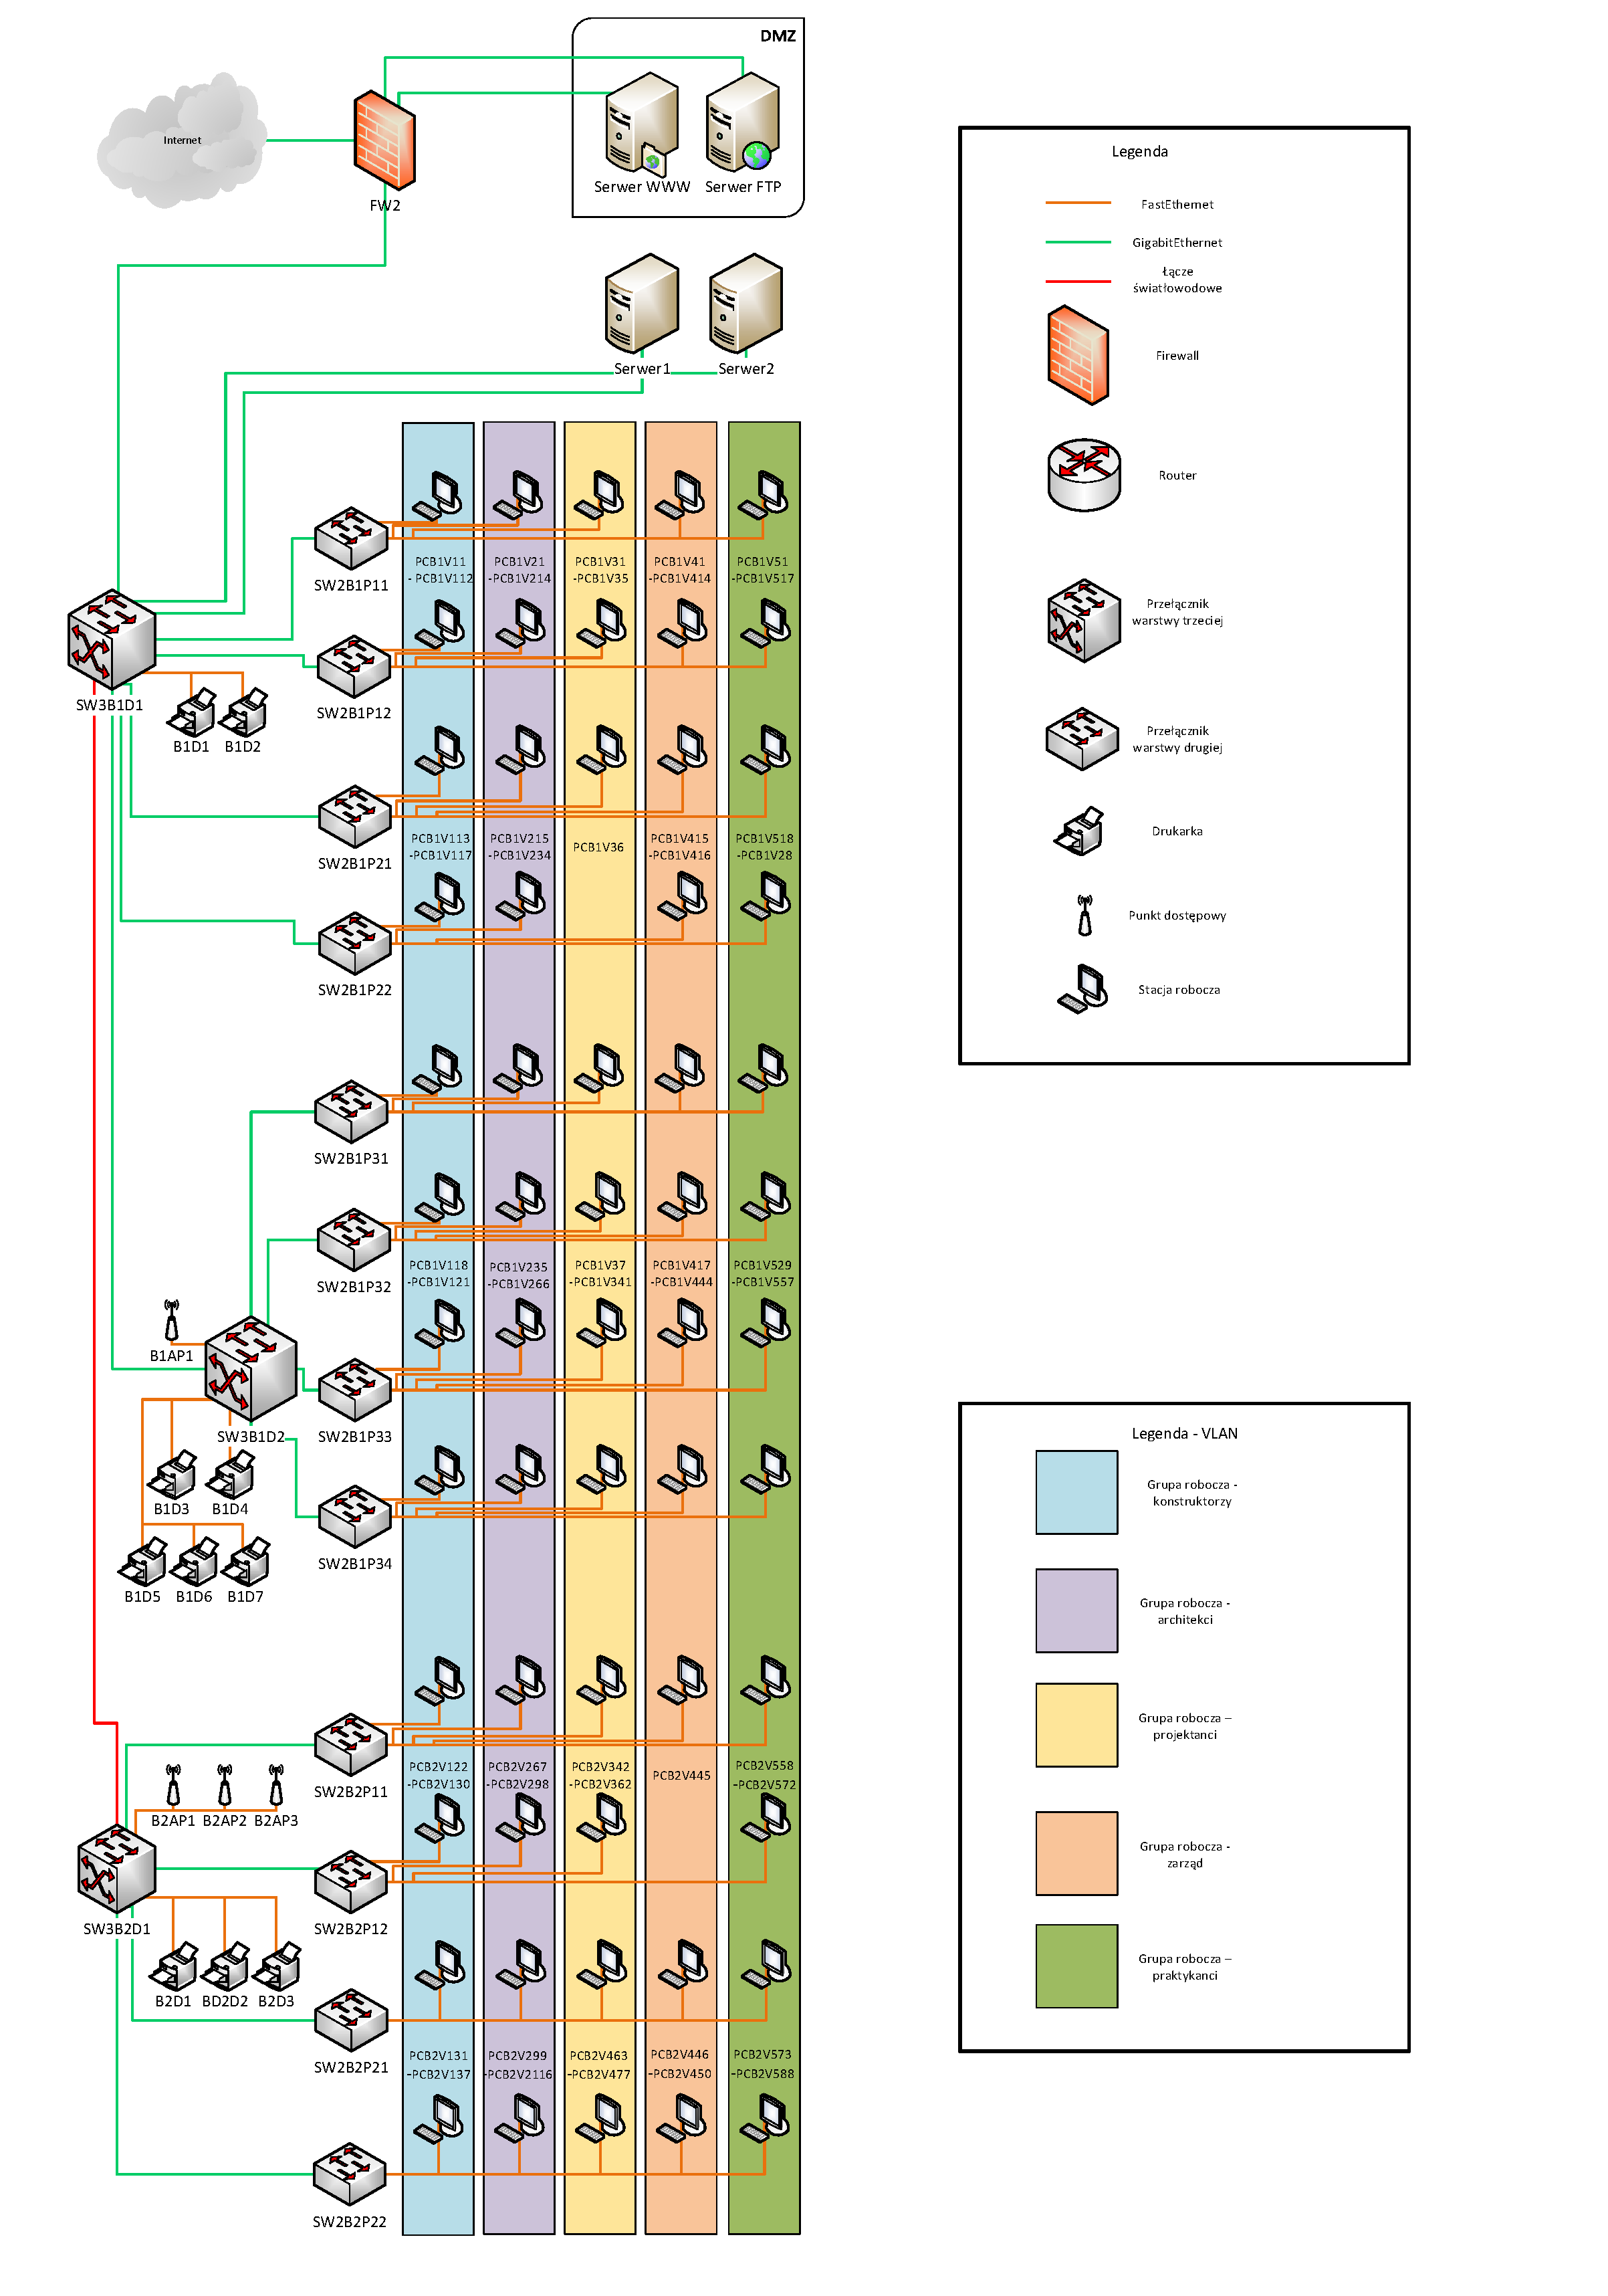
\includepdf[pages={-}]{log2.pdf}
\newpage

\begin{table}[H]
\centering
\begin{tabular}{|c|c|}
\hline
\textbf{Nazwa urzadzenia} & \textbf{Typ urządzenia}                                      \\ \hline
SW2B1P1{[}1-2{]}          & \multirow{5}{*}{switch warstwy 2.}                           \\ \cline{1-1}
SW2B1P2{[}1-2{]}          &                                                              \\ \cline{1-1}
SW2B1P3{[}1-4{]}          &                                                              \\ \cline{1-1}
SW2B2P1{[}1-2{]}          &                                                              \\ \cline{1-1}
SW2B2P2{[}1-2{]}          &                                                              \\ \hline
SW3B1D1                   & \multirow{3}{*}{switch warstwy 3.}                           \\ \cline{1-1}
SW3B1D2                   &                                                              \\ \cline{1-1}
SW3B2D1                   &                                                              \\ \hline
PCB1V1{[}1-21{]}          & \multirow{10}{*}{stacje robocze}                             \\ \cline{1-1}
PCB2V1{[}22-37{]}         &                                                              \\ \cline{1-1}
PCB1V2{[}1-66{]}          &                                                              \\ \cline{1-1}
PCB2V2{[}67-116{]}        &                                                              \\ \cline{1-1}
PCB1V3{[}1-41{]}          &                                                              \\ \cline{1-1}
PCB2V3{[}42-77{]}         &                                                              \\ \cline{1-1}
PCB1V4{[}1-44{]}          &                                                              \\ \cline{1-1}
PCB2V4{[}45-50{]}         &                                                              \\ \cline{1-1}
PCB1V5{[}1-57{]}          &                                                              \\ \cline{1-1}
PCB2V5{[}58-88{]}         &                                                              \\ \hline
R1                        & router                                                       \\ \hline
B1D{[}1-7{]}              & \multirow{2}{*}{drukarki}                                    \\ \cline{1-1}
B2D{[}1-3{]}              &                                                              \\ \hline
FW{[}1-2{]}               & firewall                                                     \\ \hline
Serwer{[}1-2{]}           & \multirow{3}{*}{serwery}                                     \\ \cline{1-1}
SerwerWWW                 &                                                              \\ \cline{1-1}
SerwerFTP                 &                                                              \\ \hline
B1AP1                     & \multicolumn{1}{l|}{\multirow{2}{*}{punkty dostępowe Wi-Fi}} \\ \cline{1-1}
B2AP{[}1-3{]}             & \multicolumn{1}{l|}{}                                        \\ \hline
\end{tabular}
\caption{Wykaz urządzeń}
\end{table}

\subsection{Wybór urządzeń sieciowych}

\indent Urządzenia wybrane do stworzenia sieci komputerowej:
\begin{enumerate}
	\item \textit{przełącznik warstwy 2.} 
	\begin{itemize}
	\item Cisco SF200-48 48-Port 10 100 Smart Switch %1 363,04 zł brutto
	\item Cisco SF200-24 24-Port 10 100 Smart Switch %775,42 zł brutto
	\end{itemize}
	
    \item \textit{przełącznik warstwy 3} 
    \begin{itemize}
	\item Cisco SG 300-20 20-port Gigabit Managed Switch
	%1 241,12 zł brutton
	\end{itemize}
    
    \item \textit{firewall} 
	\begin{itemize}
	\item ASA 5505 Appliance with SW, UL Users, 8 ports, 3DES/AES %1 954,04 zł brutto
	\end{itemize}    
    
    \item \textit{router} 
	\begin{itemize}
	\item Cisco RV325-K9-G5 Dual Gigabit WAN VPN Router %1 439,94 zł brutto
	\end{itemize}   
    
    \item \textit{serwer} 
	\begin{itemize}
	\item DELL PowerEdge T130 %3 984 zł brutto
	\end{itemize}   
   
    \item \textit{punkt dostępowy} 
	\begin{itemize}
	\item Cisco WAP4410N-G5 % 868,65 zł brutto
	\end{itemize}   
    
    \item \textit{drukarka} 
	\begin{itemize}
	\item Brother HL-1212WE WIFI %329 zł brutto
	\end{itemize}   
\end{enumerate}

\section{Projekt sieci}

\subsection{Adresacja IP}
%TODO dodać drukarki, serwery, etc.
Jako, że w zaprojektowanej przez nas sieci planujemy podział na pięć vlan-ów, tak więc na każdy vlan należy przeznaczyć osobną pulę adresów IP. Dla ułatwienia oraz biorąc pod uwagę przyszły rozwój sieci, każdy vlan będzie miał swoją pulę z maską sieci 255.255.255.0. Adresy IP zostaną przydzielone w następujący sposób:

\begin{itemize}
\item vlan10 - pula adresów 10.0.0.0 /24 (kostruktorzy) 
\item vlan20 - pula adresów 10.0.1.0 /24(architekci)
\item vlan30 - pula adresów 10.0.2.0 /24(projektanci)
\item vlan40 - pula adresów 10.0.3.0 /24(zarząd)
\item vlan50 - pula adresów 10.0.4.0 /24(praktykanci)
\end{itemize}

Sieci vlan stworzone w ten sposób będą łatwe w utrzymaniu oraz biorąc pod uwagę rozwój firmy nie będą sprawiać problemów przy zatrudnianiu nowych pracowników.

Przy zastosowaniu powyższej puli adresów, adresy przydzielone poszczególnym stacjom roboczym na konkretnych piętrach przedstawiać się będą następująco:

\begin{itemize}
\item budynek pierwszy, piętro pierwsze:
	\begin{itemize}
	\item PCB1V11 - PCB1V112 10.0.0.1 - 10.0.0.12
	\item PCB1V21 - PCB1V214 10.0.1.1 - 10.0.1.14
	\item PCB1V31 - PCB1V35 10.0.2.1 - 10.0.2.5
	\item PCB1V41 - PCB1V414 10.0.3.1 - 10.0.3.14
	\item PCB1V51 - PCB1V517 10.0.4.1 - 10.0.4.17
	\end{itemize}
\item budynek pierwszy, piętro drugie:
	\begin{itemize}
	\item PCB1V113 - PCB1V117 10.0.0.13 - 10.0.0.17
	\item PCB1V15 - PCB1V234 10.0.1.15 - 10.0.1.34
	\item PCB1V36 - 10.0.2.6
	\item PCB1V415 - PCB1V416 10.0.3.15 - 10.0.3.16
	\item PCB1V518 - PCB1V528 10.0.4.18 - 10.0.4.28
	\end{itemize}
\item budynek pierwszy, piętro trzecie:
	\begin{itemize}
	\item PCB1V118 - PCB1V121 10.0.0.18 - 10.0.0.21
	\item PCB1V235 - PCB1V266 10.0.1.35 - 10.0.1.66
	\item PCB1V37 - PCB1V341 10.0.2.7 - 10.0.2.41
	\item PCB1V417 - PCB1V444 10.0.3.17 - 10.0.3.44
	\item PCB1V529 - PCB1V557 10.0.4.29 - 10.0.4.57
	\end{itemize}
\item budynek drugi, piętro pierwsze:
	\begin{itemize}
	\item PCB1V122 - PCB1V130 10.0.0.22 - 10.0.0.30
	\item PCB1V267 - PCB1V298 10.0.1.67 - 10.0.1.98
	\item PCB1V342 - PCB1V362 10.0.2.42 - 10.0.2.62
	\item PCB1V445 - 10.0.3.45
	\item PCB1V558 - PCB1V572 10.0.4.58 - 10.0.4.72
	\end{itemize}
\item budynek drugi, piętro drugie:
	\begin{itemize}
	\item PCB1V131 - PCB1V137 10.0.0.31 - 10.0.0.37
	\item PCB1V299 - PCB1V2116 10.0.1.99 - 10.0.1.116
	\item PCB1V63 - PCB1V377 10.0.2.63 - 10.0.2.77
	\item PCB1V446 - PCB1V450 10.0.3.46 - 10.0.3.50
	\item PCB1V573 - PCB1V588 10.0.4.73 - 10.0.4.88
	\end{itemize}
\end{itemize}

\subsection{Projekt konfiguracji urządzeń}
Stworzone przez nas vlany oparte będą o standard 802.1q. Aby poprawnie skonfigurować interfejsy na przełącznikach, trzeba wiedzieć, do których portów podłączone będą komputery na poszczególnych przełącznikach, oraz które porty służyć będą do utworzenia łącz trunkingowych. Stacje robocze zostaną podłączone do przerzutników w następujący sposób:

\begin{itemize}
\item SW2B1P11:
	\begin{itemize}
	\item porty 1 - 12 PCB1V11 - PCB1V112, vlan10 
	\item porty 13 - 26 PCB1V21 - PCB1V214, vlan20
	\item porty 27 - 31 PCB1V31 - PCB1V35, vlan30
	\item port 48 trunk
	\end{itemize}
\item SW2B1P12:
	\begin{itemize}
	\item porty 1 - 14 PCB1V41 - PCB1V414, vlan40
	\item porty 15 - 31 PCB1V51 - PCB1V517, vlan50
	\item port 48 trunk
	\end{itemize}
	
\item SW2B1P21:
	\begin{itemize}
	\item porty 1 - 5 PCB1V113 - PCB1V117 vlan10
	\item porty 6 - 25 PCB1V15 - PCB1V234 vlan20
	\item port 26 PCB1V36 vlan30
	\item port 48 trunk
	\end{itemize}
\item SW2B1P22:
	\begin{itemize}
	\item porty 1 - 2 PCB1V415 - PCB1V416 vlan40
	\item porty 3 - 13 PCB1V518 - PCB1V528 vlan50
	\item port 24 trunk
	\end{itemize}
\item SW2B1P31:
	\begin{itemize}
	\item porty 1 - 4 PCB1V118 - PCB1V121 vlan10
	\item porty 4 - 32 PCB1V417 - PCB1V444 vlan40
	\item port 48 trunk
	\end{itemize}
\item SW2B1P32:
	\begin{itemize}
	\item porty 1 - 32 PCB1V235 - PCB1V266 vlan20
	\item port 48 trunk
	\end{itemize}
\item SW2B1P33:
	\begin{itemize}
	\item porty 1 - 35 PCB1V37 - PCB1V341 vlan30
	\item port 48 trunk
	\end{itemize}
\item SW2B1P34:
	\begin{itemize}
	\item porty 1 - 29 PCB1V529 - PCB1V557 vlan50
	\item port 48 trunk
	\end{itemize}
	
\item SW2B2P11:
	\begin{itemize}
	\item porty 1 - 9 PCB1V122 - PCB1V130 vlan10
	\item porty 10 - 41 PCB1V267 - PCB1V298 vlan20
	\item port 42 PCB1V445 vlan40
	\item port 48 trunk
	\end{itemize}
	
\item SW2B2P12:
	\begin{itemize}
	\item porty 1 - 21 PCB1V342 - PCB1V362 vlan30
	\item porty 22 - 36 PCB1V558 - PCB1V558 vlan50
	\item port 48 trunk
	\end{itemize}
	
\item SW2B2P21:
	\begin{itemize}
	\item porty 1 - 7 PCB1V131 - PCB1V137 vlan10
	\item porty 8 - 25 PCB1V299 - PCB1V2116 vlan20
	\item porty 26 - 42 PCB1V63 - PCB1V377 vlan30
	\item port 48 trunk
	\end{itemize}
	
\item SW2B2P22:
	\begin{itemize}
	\item porty 1 - 5 PCB1V446 - PCB1V450 vlan40
	\item porty 6 - 21 PCB1V573 - PCB1V588 vlan50
	\item port 24 trunk
	\end{itemize}

\item SW3B1D1:
	\begin{itemize}
	\item porty 19, 20, 21, 22, 23, 24 trunk
	\item porty 1,2 - B1D1, B2D2 (drukarki)
	\end{itemize}
	
\item SW3B1D2:
	\begin{itemize}
	\item porty 20, 21, 22, 23, 24 trunk
	\item porty 1,2,3,4,5 - B1D3 - B2D7 (drukarki)
	\item port 6 - B1AP1 (access point)
	\end{itemize}
	
\item SW3B2D1:
	\begin{itemize}
	\item porty 20, 21, 22, 23, 24 trunk
	\item porty 1,2,3 - B1D1 - B2D3 (drukarki)
	\item porty 4,5,6 - B2AP1 - B2AP3 (access point)
	\end{itemize}
	
\end{itemize}

\subsection{Projekt podłączenia do Internetu}

\subsection{Analiza bezpieczeństwa i niezawodności sieci}
Prezentowany przez nas projekt zakłada wykorzystanie pewnych mechanizmów zapewniających lepsze bezpieczeństwo sieci. Aby zabezpieczyć sieć lokalną przed nieautoryzowanym dostępem osób trzecich z zewnątrz, sieć wyposażona będzie w firewall. W niezawodności sieci istotną rolę gra odporność na czynniki zewnętrzne, takie jak chwilowe przerwy w dostawie zasilania. Wprawdzie umowa, jaką dostawca prądu podpisuje z klientem, zapewniona jest pewna niezawodność, niemniej jednak chwilowe awarie prądu mogą stanowić zagrożenie dla danych znajdujących się na serwerze. Biorąc ten czynnik pod uwagę, zdecydowaliśmy się wyposażyć sieć lokalną w zasilacz UPS, który w razie krótszych awarii zasilania utrzyma pracę serwera, a w przypadku dłuższych awarii pozwoli na bezpieczne wyłączenie serwerów bez obawy o utratę danych. Do tego celu zastosowany zostanie zasilacz \textit{UPS Liebert PSI 750VA}.%1631.84 PLN brutto
Serwery WWW i FTP umieszczone zostaną w strefie zdemilitaryzowanej (DMZ).

\subsection{Kosztorys}

Koszty urządzeń potrzebnych do funkcjonowania sieci przedstawiają się następująco:
\begin{enumerate}
	\item \textit{przełącznik warstwy 2.} 
	\begin{itemize}
	\item Cisco SF200-48 48-Port 10 100 Smart Switch * 10 = 1363,04 zł * 10 = 13630,04 zł brutto
	\item Cisco SF200-24 24-Port 10 100 Smart Switch * 2 = 775,42 zł * 2 = 1550,84 zł brutto
	\end{itemize}
	
    \item \textit{przełącznik warstwy 3} 
    \begin{itemize}
	\item Cisco SG 300-20 20-port Gigabit Managed Switch * 4 = 1241,12 zł * 4 = 4964,48 zł brutto
	%1 241,12 zł brutton
	\end{itemize}
    
    \item \textit{firewall} 
	\begin{itemize}
	\item ASA 5505 Appliance with SW, UL Users, 8 ports, 3DES/AES = 1954,04 zł brutto
	\end{itemize}    
    
    \item \textit{router} 
	\begin{itemize}
	\item Cisco RV325-K9-G5 Dual Gigabit WAN VPN Router = 1439,94 zł brutto
	\end{itemize}   
    
    \item \textit{serwer} 
	\begin{itemize}
	\item DELL PowerEdge T130 * 4 = 3984 zł * 4 = 15936 zł brutto
	\end{itemize}   
   
    \item \textit{punkt dostępowy} 
	\begin{itemize}
	\item Cisco WAP4410N-G5 * 4 = 868,65 zł * 4 =  3474,6 zł brutto
	\end{itemize}   
    
    \item \textit{drukarka} 
	\begin{itemize}
	\item Brother HL-1212WE WIFI * 10 = 3290 zł brutto
	\end{itemize}

	\item \textit{UPS} 
	\begin{itemize}
	\item Zasilacz awaryjny UPS Liebert PSI 750VA = 1631,84 zł brutto
	\end{itemize}  
\end{enumerate}

Wszystko daje całkowity koszt 13630,04 + 1550,84 + 4964,48 + 1954,04 + 1439,94 + 
15936 + 3474,6 + 3290 + 1631,84 = 47871,78 zł.

Uwzględniając koszt dwuletniego opłacenia umowy z dostawcą sieci internet - 1320 złotych, koszt całkowity wyniesie 49191,78 zł.

\subsection*{Dostawca dostępu sieci Internet}
\indent Dostawca sieci Internet został wybrany na podstawie maksymalnego transferu generowanego przez aplikacje komputerowe. Jako że download i upload są zbliżone do siebie wykorzystane zostanie \textbf{łącze symetryczne}.
\newline \indent Po analizie rynku dostawców wytypowana została firma \textbf{Moico}, która w swojej ofercie ma dostępny odpowiedni model. Pakiet, który spełnia minimalne wymagania, a nawet zapewni pewną nadmiarowość transferu, to \textbf{KISS}. Prędkość łącza we wspomnianym pakiecie wynosi \textbf{100 Mbps}, a umowa jest na czas nieokreślony. Cena utrzymania miesięcznie wynosi \textbf{55 zł}, co przy umowie na 2 lata da 55 zł $\cdot$ 12 mies. $\cdot$ 2 lata = \textbf{1320 zł}.    

%TODO dodać koszt internetu na 2 lata :d

\section{Karty katalogowe proponowanych urządzeń}
\subsection{Przełącznik warstwy drugiej}
\begin{figure}[H]
\centering
    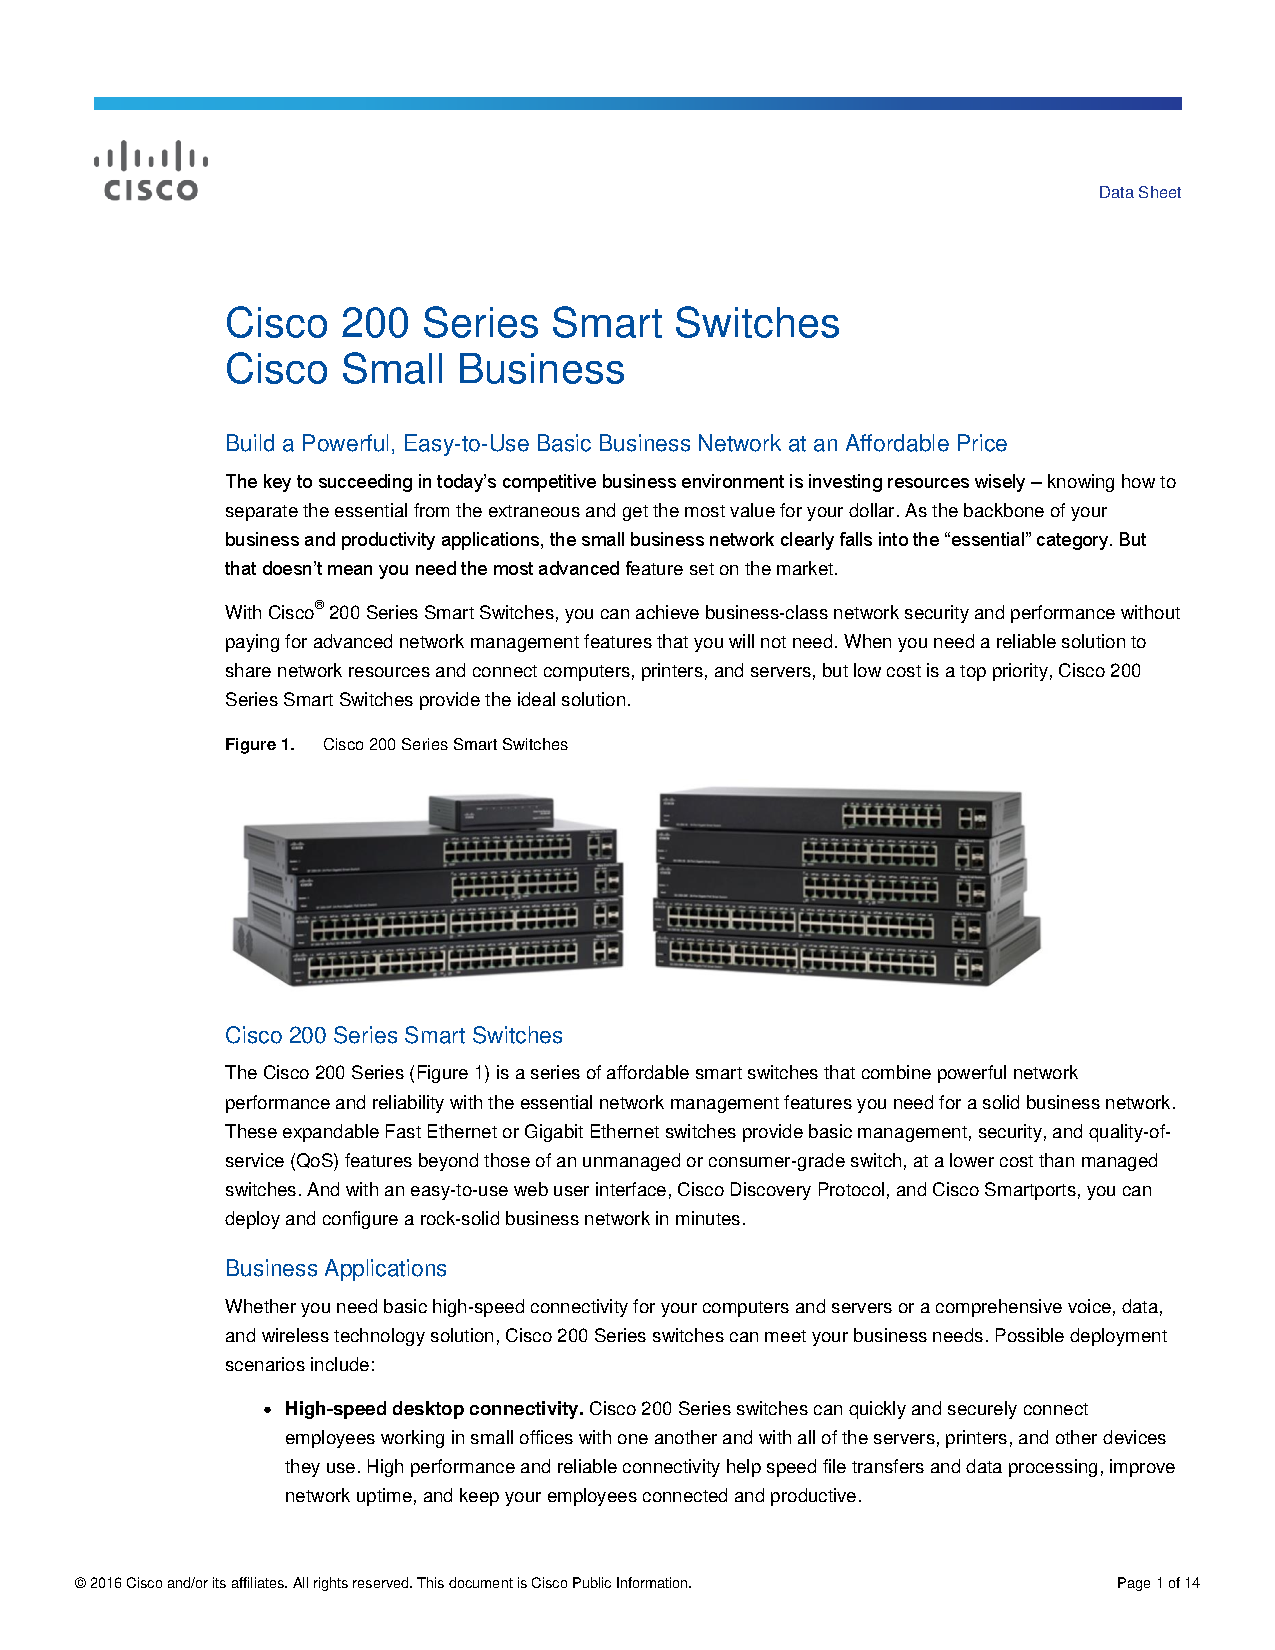
\includegraphics[scale=0.80]{spec/sw2.pdf}%<---angle here
    \label{fig:PropProf}
\end{figure}

\subsection{Przełącznik warstwy trzeciej}
\begin{figure}[H]
\centering
    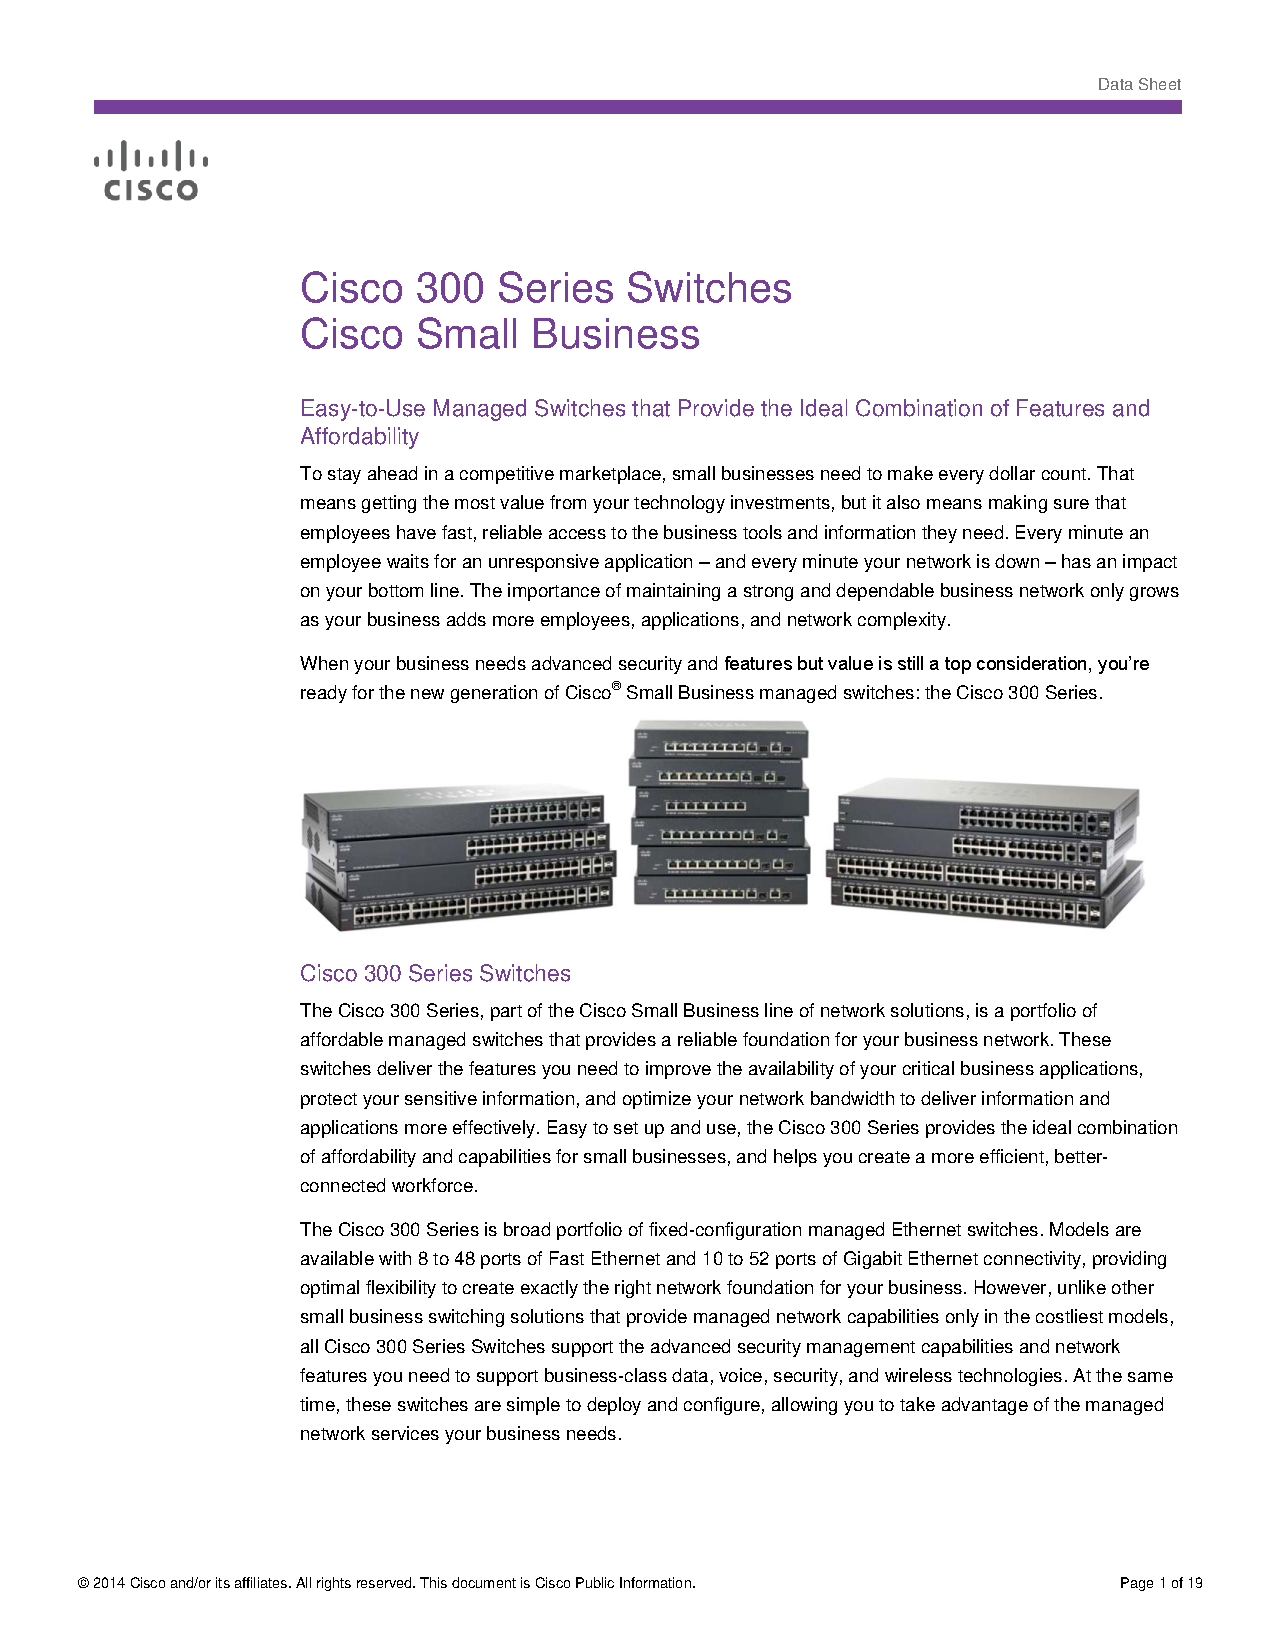
\includegraphics[scale=0.80]{spec/sw3.pdf}%<---angle here
    \label{fig:PropProf}
\end{figure}

\subsection{Firewall}
\begin{figure}[H]
\centering
    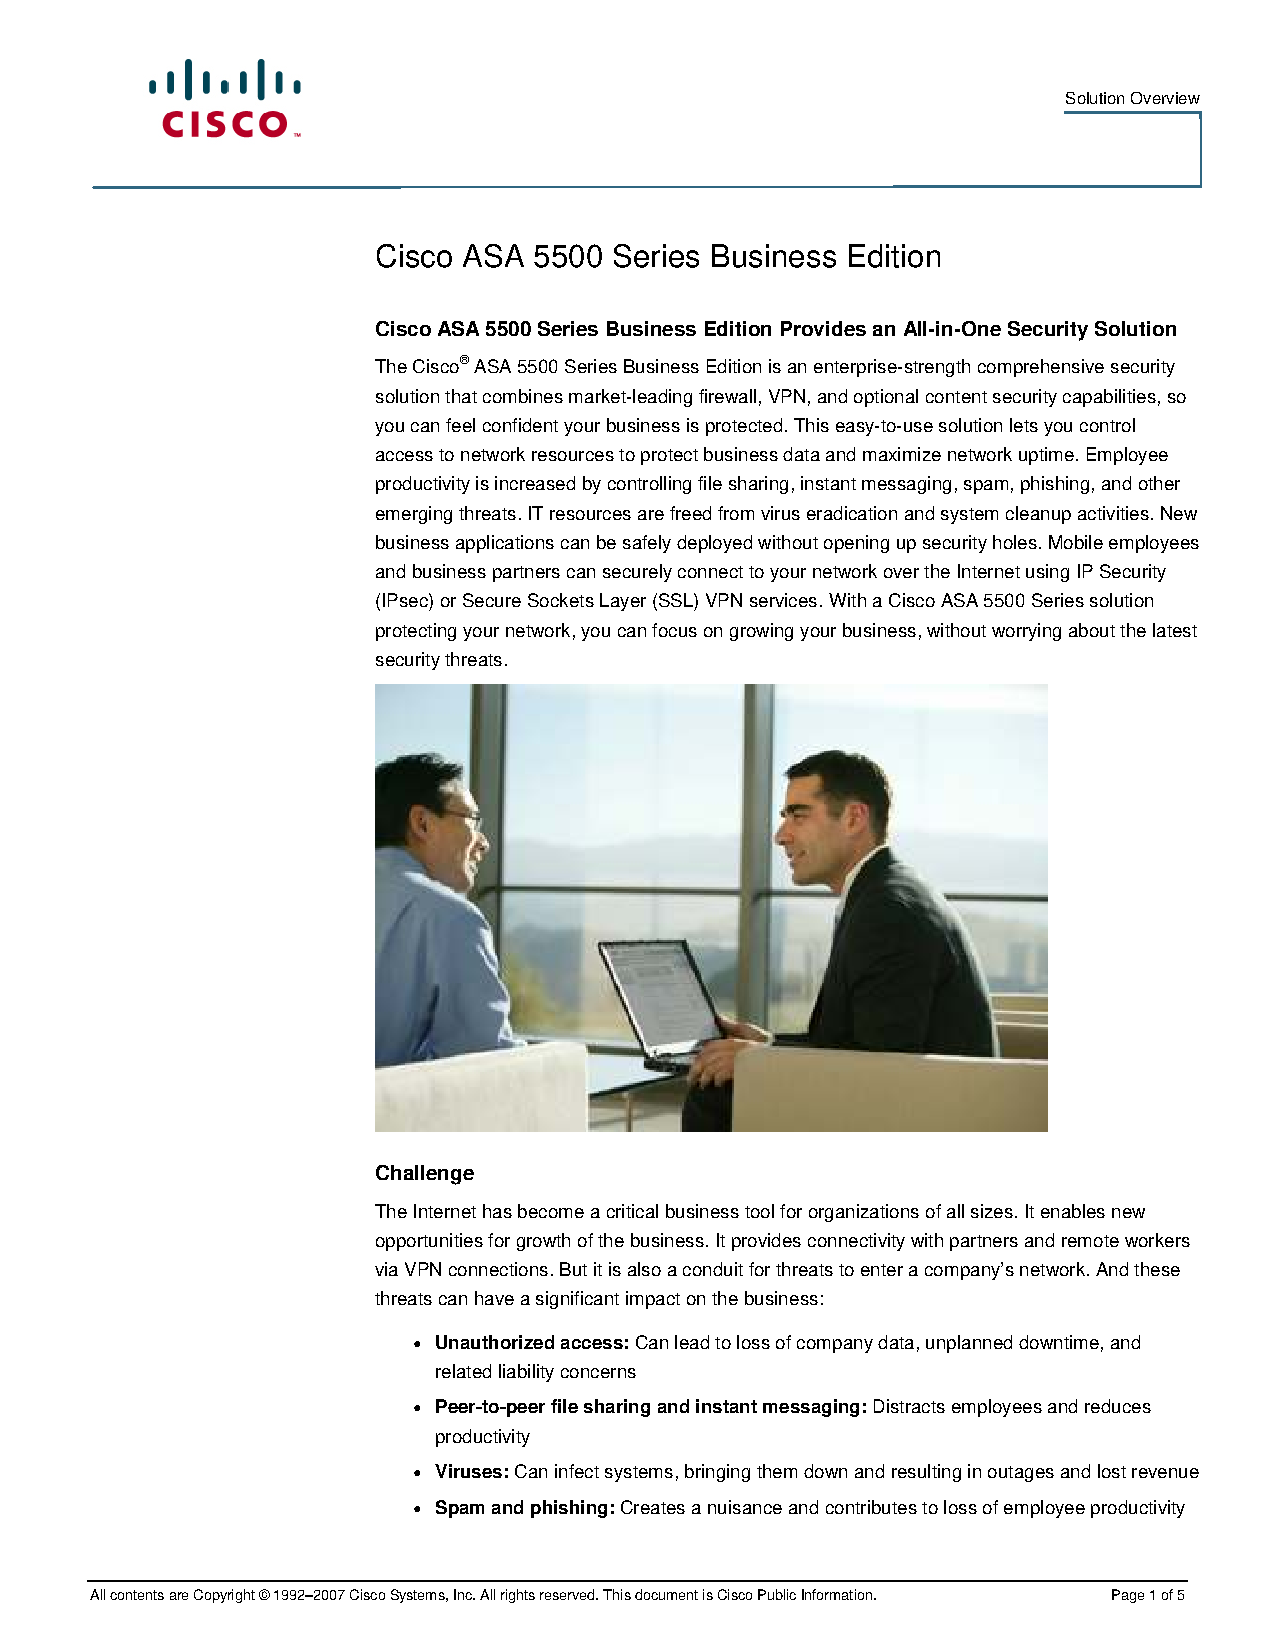
\includegraphics[scale=0.80]{spec/firewall.pdf}%<---angle here
    \label{fig:PropProf}
\end{figure}

\subsection{Router}
\begin{figure}[H]
\centering
    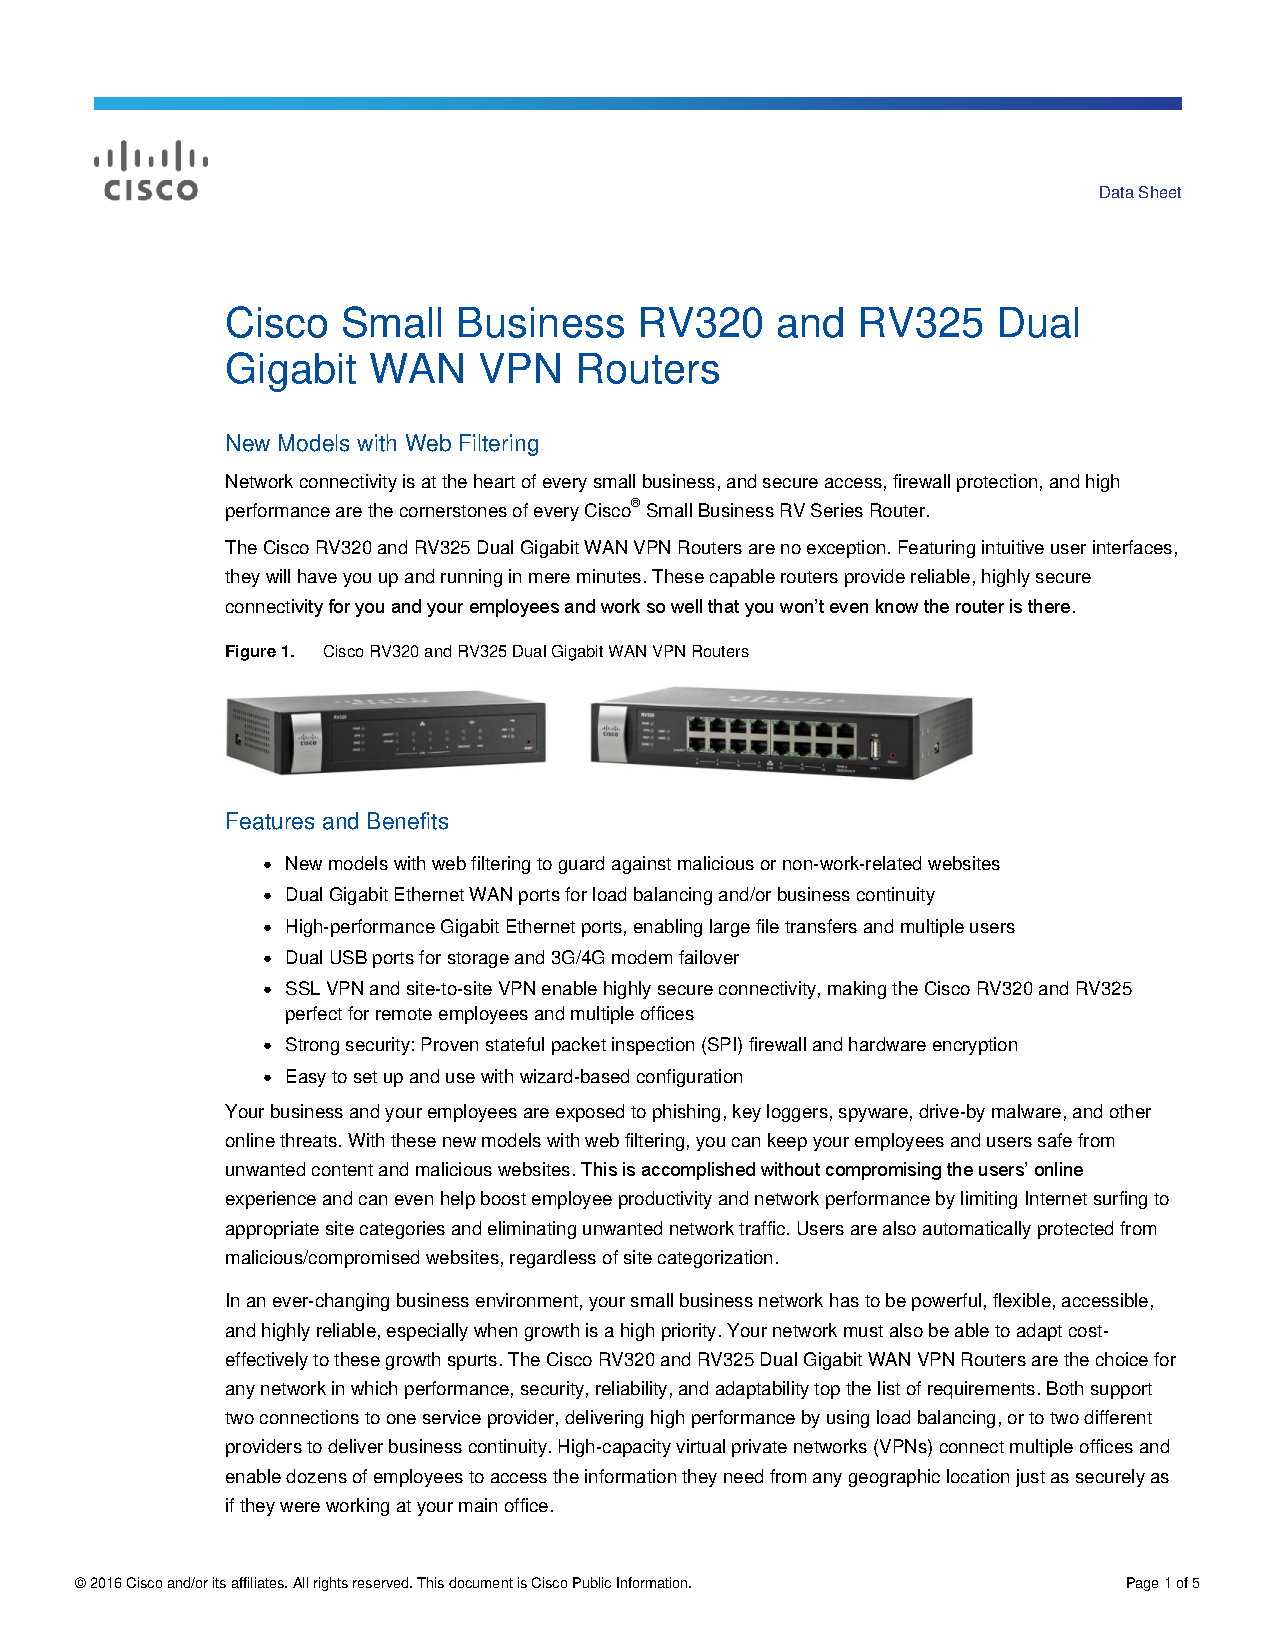
\includegraphics[scale=0.80]{spec/router.pdf}%<---angle here
    \label{fig:PropProf}
\end{figure}

\subsection{Serwer}
\begin{figure}[H]
\centering
    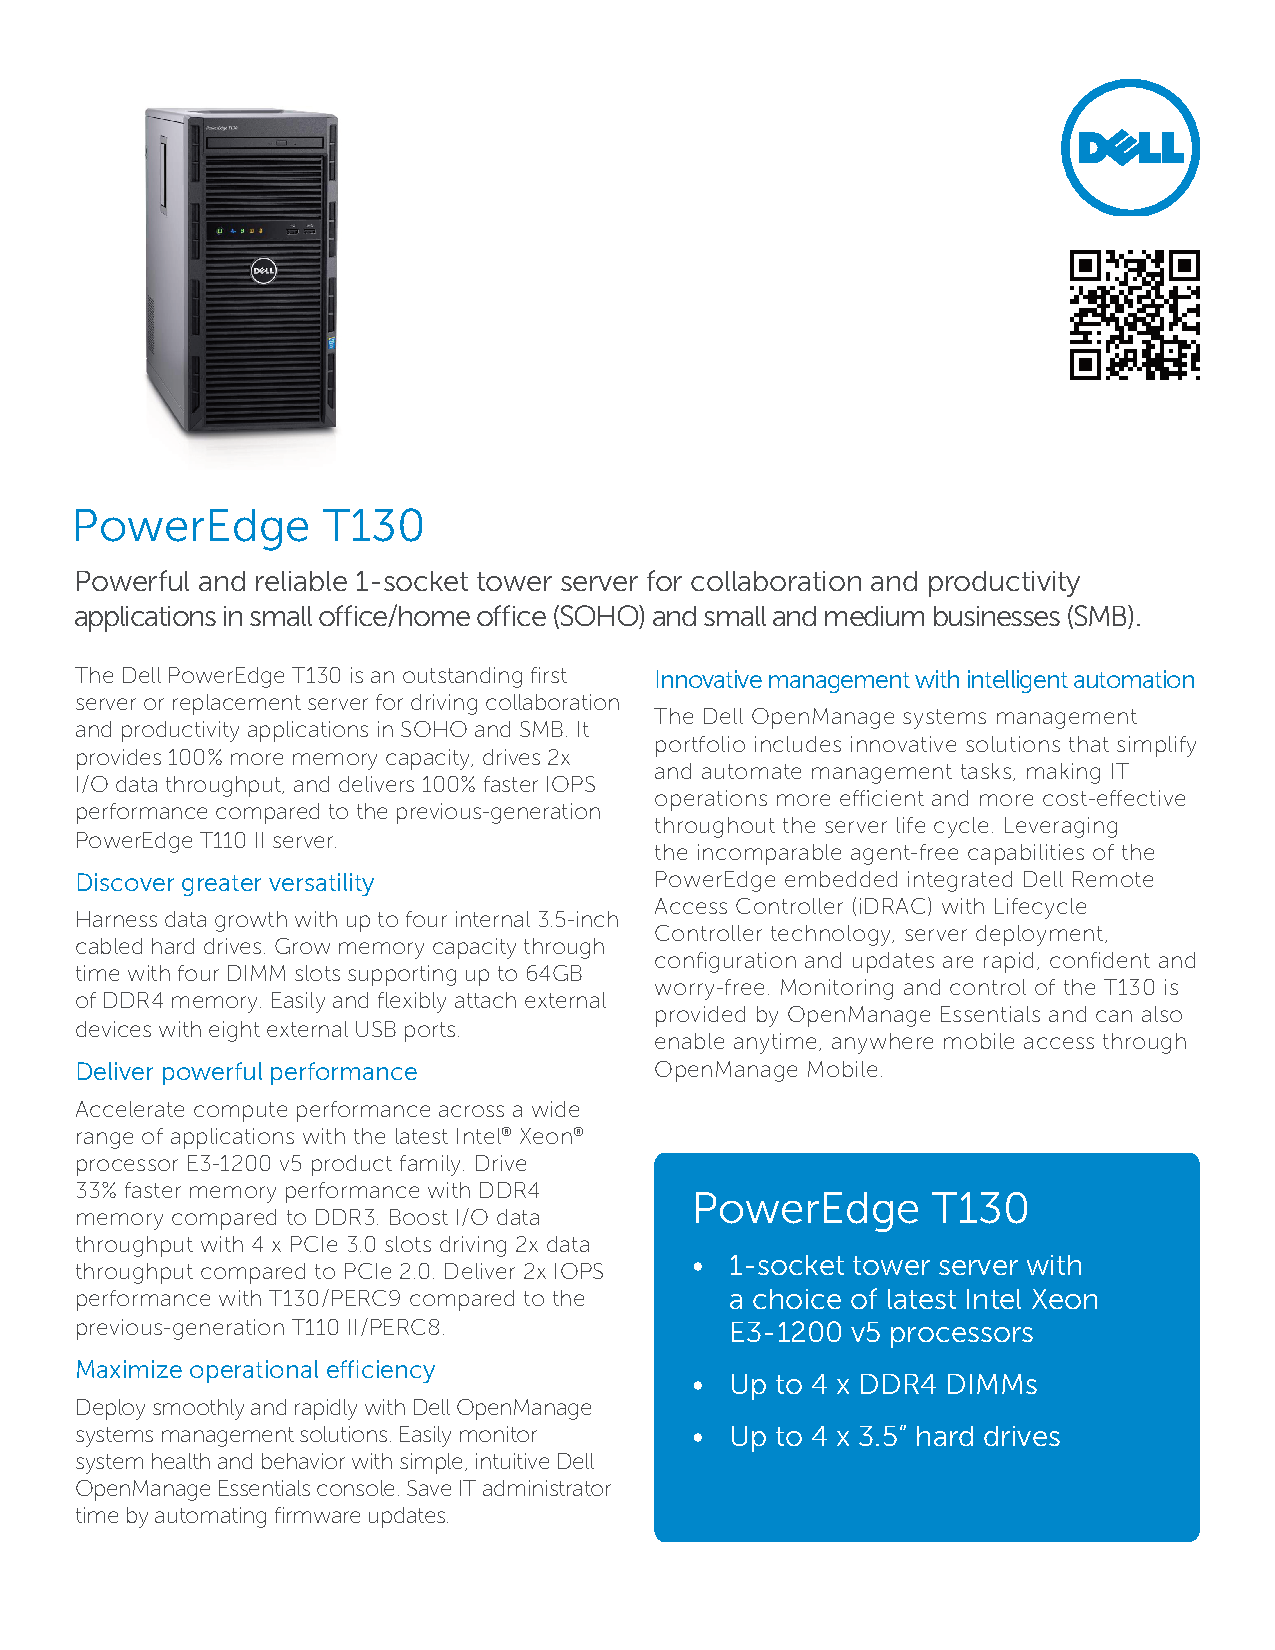
\includegraphics[scale=0.80]{spec/serwer.pdf}%<---angle here
    \label{fig:PropProf}
\end{figure}

\subsection{Punkty dostępowe}
\begin{figure}[H]
\centering
    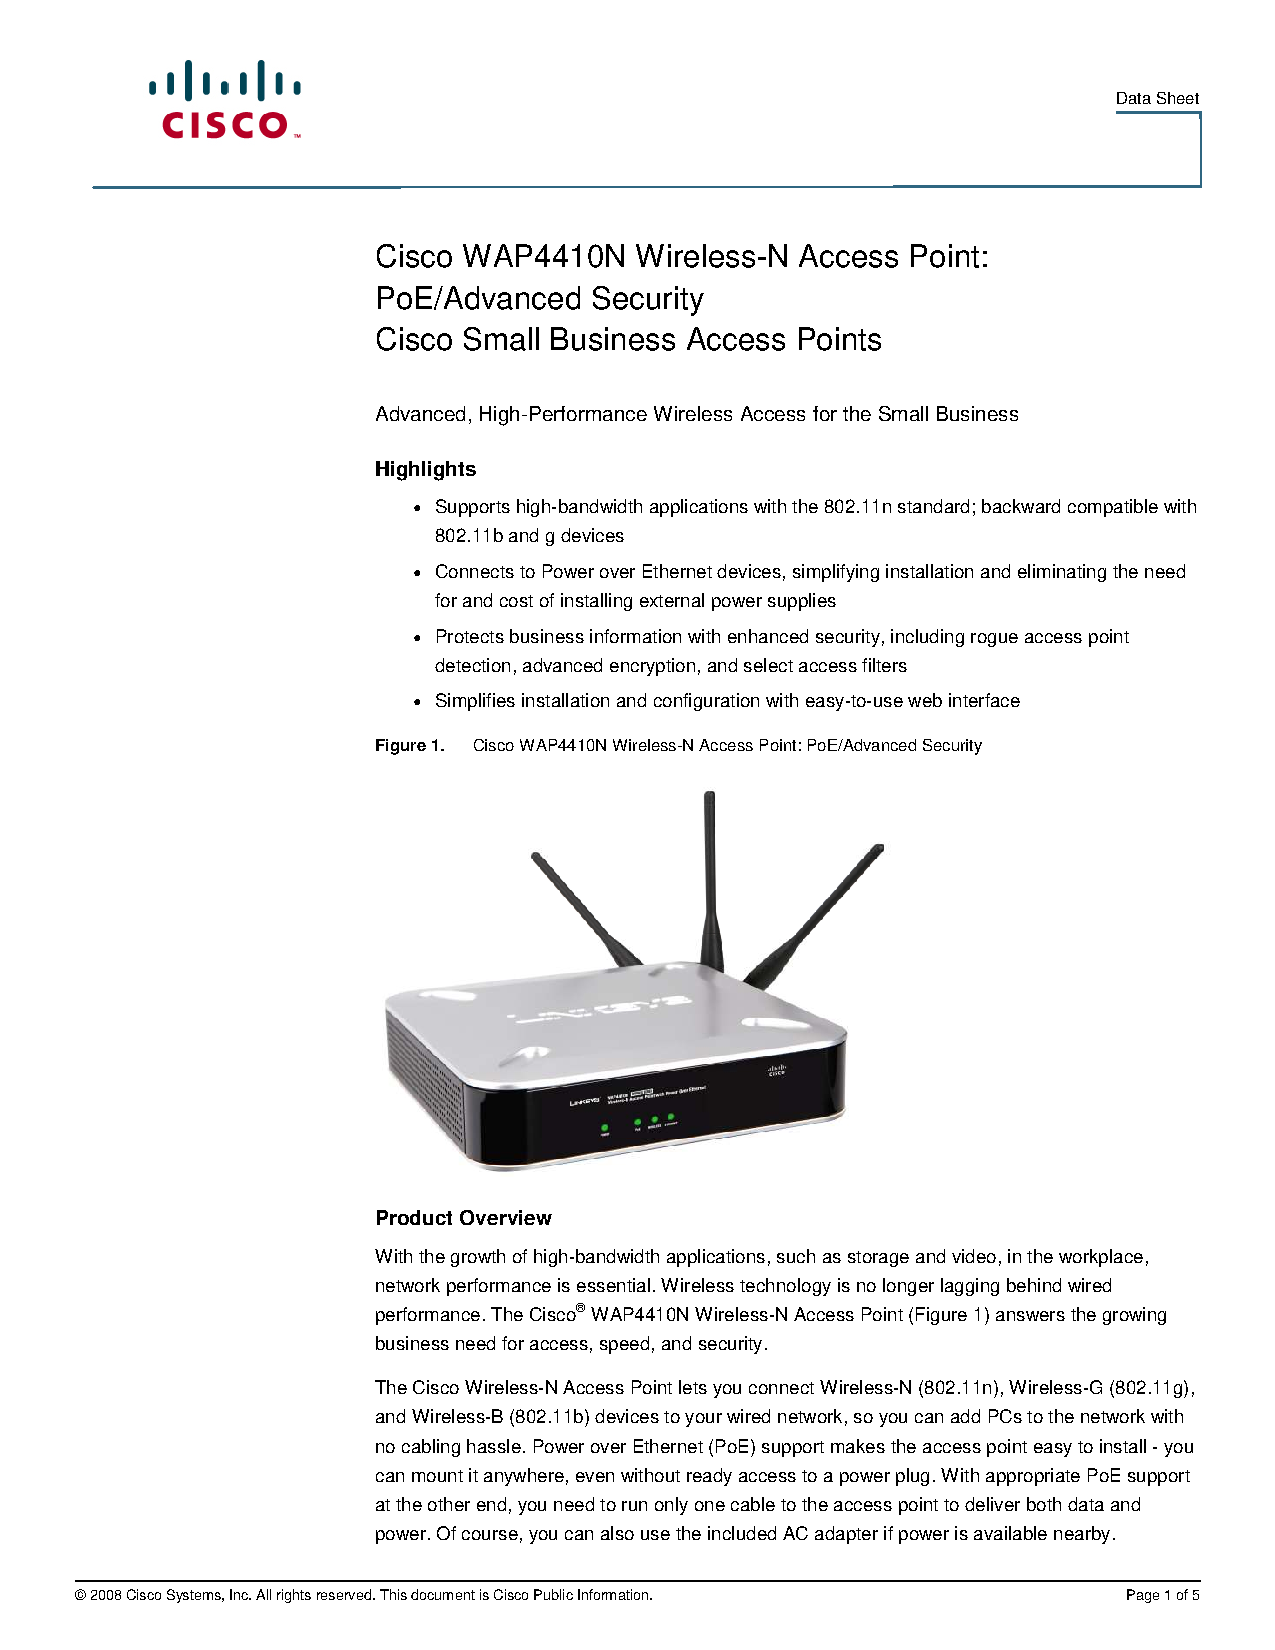
\includegraphics[scale=0.80]{spec/access.pdf}%<---angle here
    \label{fig:PropProf}
\end{figure}

\subsection{UPS}
\begin{figure}[H]
\centering
    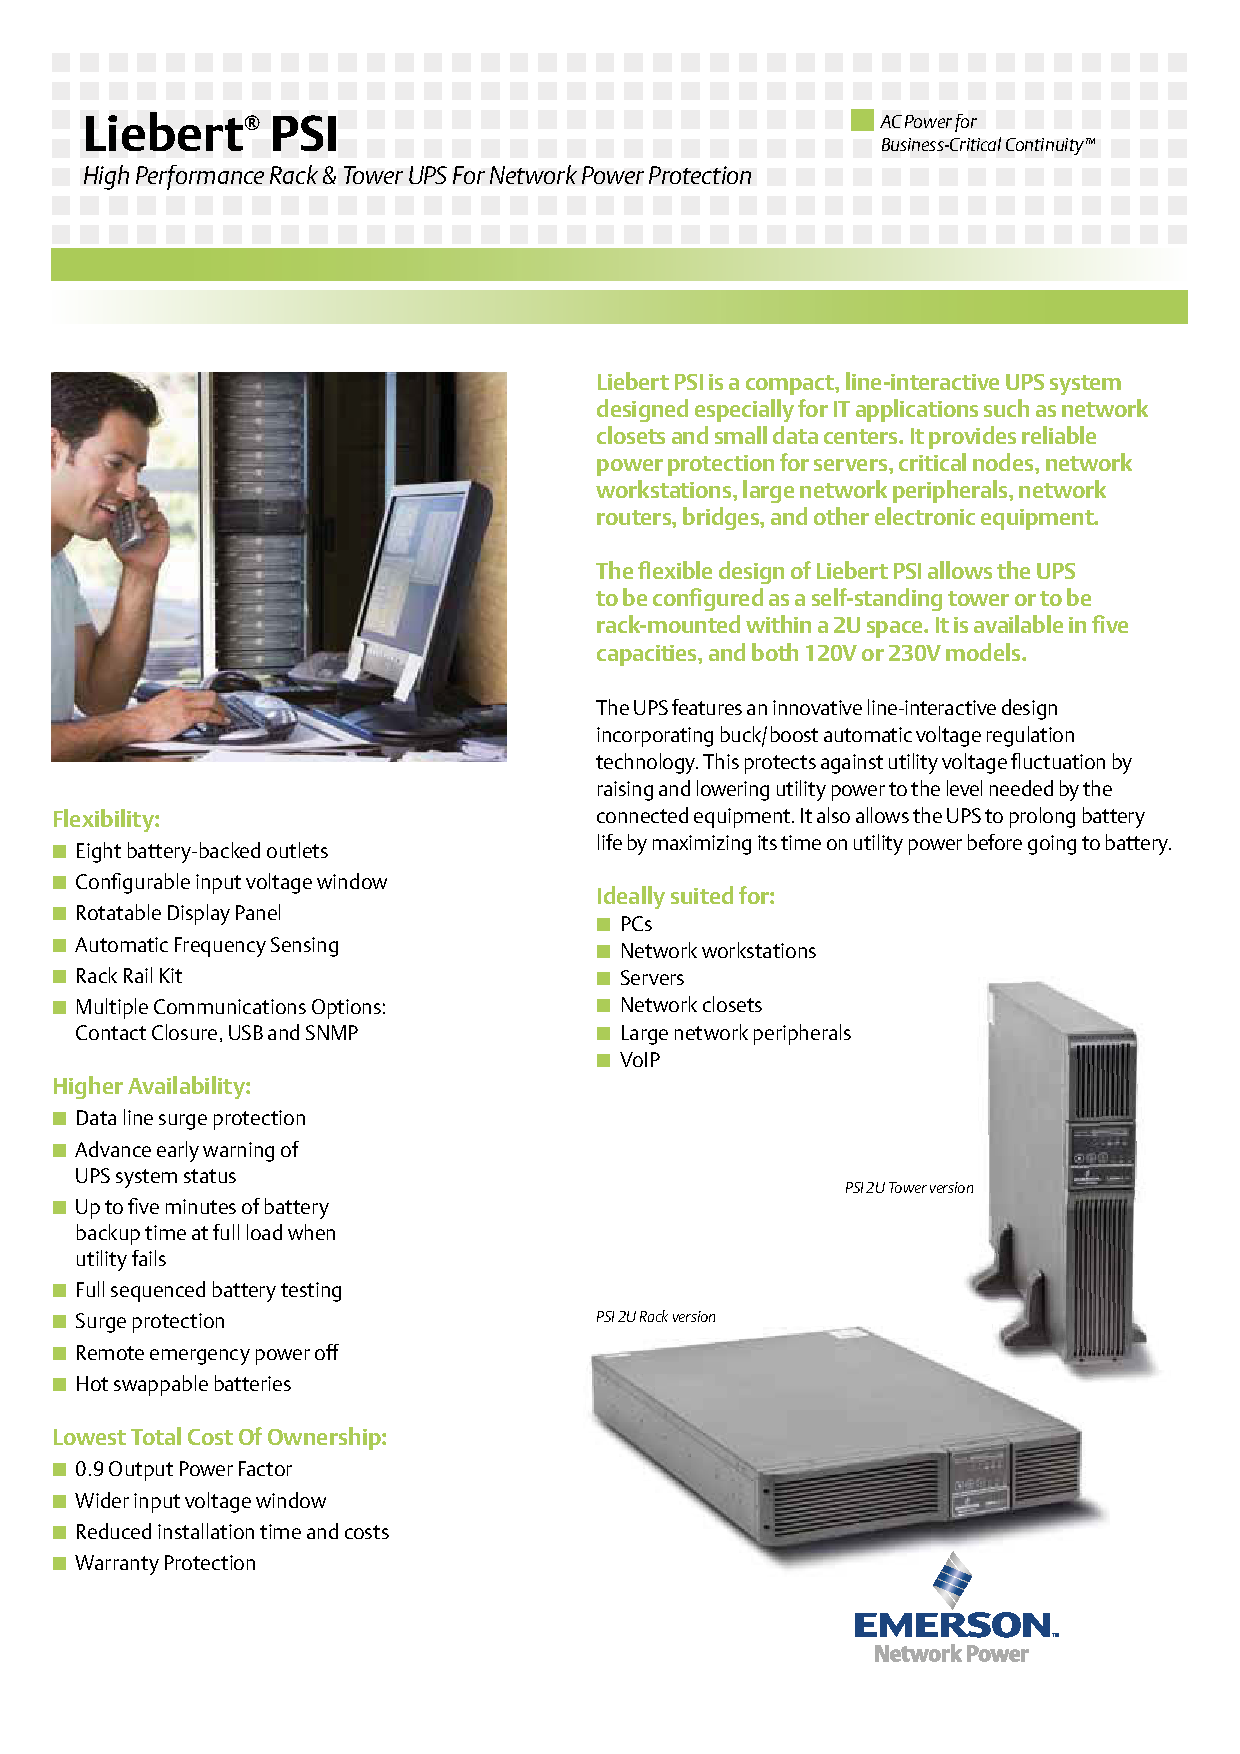
\includegraphics[scale=0.80]{spec/ups.pdf}%<---angle here
    \label{fig:PropProf}
\end{figure}

Przełącznik warstwy 2.
Switche - 
\\\url{http://www.cisco.com/c/en/us/products/collateral/switches/small-business-200-series-smart-switches/data_sheet_c78-634369.html}

Przełącznik warstwy 3.
\\\url{http://www.cisco.com/c/en/us/products/collateral/switches/small-business-smart-switches/data_sheet_c78-610061.html}

Firewall
\\\url{http://www.cisco.com/c/en/us/support/security/asa-5505-adaptive-security-appliance/model.html}

Router
\\\url{http://www.cisco.com/c/en/us/products/collateral/routers/rv325-dual-gigabit-wan-vpn-router/datasheet-c78-729726.html}

Serwer
\\\url{http://i.dell.com/sites/doccontent/shared-content/data-sheets/en/Documents/Dell_PowerEdge_T130_SpecSheet_final.pdf?newtab=true}

Access Point
\\\url{http://www.cisco.com/c/en/us/products/collateral/wireless/small-business-wireless-access-points/data_sheet_c78-501860.html}

Drukarka
\\\url{http://support.brother.com/g/b/spec.aspx?c=gb&lang=en&prod=hl1212w_us_eu}

UPS
\\\url{http://www.powerserver.pl/d8687_zasilacz_awaryjny_ups_liebert_psi_750va.html#specyfikacja}

\end{document}